\documentclass[conference]{IEEEtran}
\IEEEoverridecommandlockouts
\usepackage[T1]{fontenc}
\usepackage[utf8]{inputenc}
\usepackage{babel}
\babelprovide[import,main]{italian}
\usepackage{amsmath,amssymb}
\usepackage{graphicx}
\usepackage{booktabs,tabularx,array}
\usepackage{listings,xcolor}
\usepackage[section]{placeins}
\usepackage{flafter}
\usepackage{balance}
\usepackage{url}
\usepackage[hidelinks]{hyperref}
\lstset{basicstyle=\ttfamily\scriptsize,breaklines=true,columns=fullflexible,
 keepspaces=true,showstringspaces=false,frame=single,captionpos=b}
\newcommand{\code}[1]{\texttt{\detokenize{#1}}}
\renewcommand{\lstlistingname}{Listato}
\begin{document}
\raggedbottom
\title{SLM isolation assessment su NVIDIA Orin AGX}
\author{\IEEEauthorblockN{Sarnataro Federica M63001769}
\IEEEauthorblockA{fed.sarnatero@studenti.unina.it}
\and\IEEEauthorblockN{Tafuri Francesco M63001712}
\IEEEauthorblockA{fran.tafuri@studenti.unina.it}}
\maketitle
\begin{abstract}
Nei sistemi embedded, la scelta di un'azione tra alternative predefinite è un problema di classificazione e non richiede necessariamente l'impiego di un modello linguistico generativo (LLM). I cosiddetti System One Models, presentati come sistemi che associano a uno stato decisioni probabilistiche, svolgono funzionalmente il ruolo di classificatori: la selezione tra classi note non costituisce di per sé una novità metodologica. Lo scopo di questo lavoro è mostrare, attraverso un confronto sperimentale, che la generazione autoregressiva non è sempre necessaria per compiti decisionali strutturati e valutarne i costi in termini di latenza e prevedibilità. Si confrontano SemIf-OpenJev, un'implementazione aperta e indipendente dell'interfaccia decisionale proposta da TypeSafe per Jev, e Gemma 4 31B quantizzato a 8 bit, impiegato in modalità generativa. SemIf utilizza Qwen3.5 4B in BF16 come classificatore: esegue un singolo passaggio e normalizza i logit associati alle alternative ammesse, senza generare token di risposta. Su NVIDIA Jetson AGX Orin, un'infrastruttura ROS 2 simula le decisioni di un robot mobile.
\end{abstract}



\FloatBarrier
\section{Infrastruttura}\label{sec:infra}

\FloatBarrier
\subsection{Obiettivo e scenario}
L'obiettivo è confrontare due approcci all'impiego di modelli linguistici in termini di responsività, stabilità, accuratezza e sensibilità alle interferenze. TypeSafe introduce la categoria \emph{System One Models} presentando Jev: sistemi che ricevono uno stato e restituiscono decisioni probabilistiche con tipi e alternative definiti dall'applicazione~\cite{typesafe}. La denominazione richiama la distinzione di Kahneman tra pensiero rapido e ragionamento deliberato. Nel presente confronto, \emph{System One} identifica l'interfaccia decisionale diretta di SemIf, mentre \emph{System Two} identifica l'impiego generativo di Gemma; si tratta di una distinzione operativa, che non implica una classificazione universale delle architetture.
SemIf, precedentemente denominato OpenJev, è un progetto aperto e indipendente che riproduce il paradigma di interfaccia di Jev mediante modelli a pesi aperti. Non è una distribuzione ufficiale del modello proprietario di TypeSafe e non ne replica l'architettura o l'addestramento~\cite{openjev}.
Lo scenario consiste nel controllo decisionale simulato di un robot mobile. A partire dalla distanza dall'ostacolo, dalla temperatura del motore e dalla velocità, il modello seleziona una delle azioni \code{proceed}, \code{slow_down} e \code{stop}. L'azione attesa è \code{stop} quando la distanza è inferiore a 0,5 m oppure la temperatura supera 90~$^\circ$C; in assenza di tali condizioni, è \code{slow_down} quando la distanza è inferiore a 1,5 m oppure la temperatura supera 75~$^\circ$C; negli altri casi è \code{proceed}.
Il requisito applicativo è di natura real-time. La valutazione sperimentale caratterizza il comportamento temporale dei modelli; i massimi osservati non costituiscono limiti superiori garantiti del tempo di esecuzione.
\FloatBarrier
\subsection{Differenze tra i modelli}
La Tabella~\ref{tab:models} riassume le configurazioni. Gemma 4 appartiene alla famiglia di modelli generativi a pesi aperti di Google; la variante 31B adotta un'architettura densa~\cite{gemma-core,gemma-card}. Nella configurazione sperimentale, Gemma elabora l'ingresso nella fase di \emph{prefill} e produce la risposta nella fase di \emph{decode}.
SemIf utilizza invece Qwen3.5 4B con pesi congelati. In modalità \code{direct}, costruisce un prompt con stato, criterio e alternative, esegue un singolo passaggio e applica una softmax ai logit dei token-lettera associati alle opzioni. Non campiona token di risposta e non esegue un ciclo di decodifica~\cite{openjev-method}. Le probabilità sono condizionate alle alternative ammesse; non equivalgono automaticamente a una confidenza calibrata. Il risultato è serializzato in JSON dal software applicativo.
Il confronto coinvolge modelli di dimensione, precisione numerica e motore di esecuzione differenti: le differenze osservate non possono essere attribuite esclusivamente alla modalità di produzione dell'output.

\begin{table}[!htbp]
\centering
\caption{Caratteristiche dei modelli confrontati.}\label{tab:models}
\footnotesize

\begin{tabularx}{\columnwidth}{l >{\raggedright\arraybackslash}X >{\raggedright\arraybackslash}X}
\toprule
Aspetto & Gemma & SemIf \\
\midrule
Input & Prompt testuale con domanda, stato e azioni & Stato, criterio e alternative descritte in JSON \\
Output & Testo generato, vincolato a uno schema JSON & Probabilità condizionate delle alternative e scelta \\
Motore & llama.cpp su GPU & PyTorch su GPU \\
Modello di base & Gemma 4 31B, quantizzato a 8 bit & Qwen3.5 4B, non quantizzato (BF16) \\
\bottomrule
\end{tabularx}
\end{table}

\FloatBarrier
\subsection{Hardware e software}
La piattaforma è una NVIDIA Jetson AGX Orin con 64 GB di memoria LPDDR5 condivisa tra CPU e GPU, CPU a 12 core Cortex-A78AE e GPU Ampere. La configurazione software è riportata nella Tabella~\ref{tab:platform}. I benchmark sono condotti con profilo energetico MAXN e frequenze di CPU e GPU impostate al massimo tramite \code{jetson_clocks}. I carichi non real-time sono generati mediante \code{stress-ng}; i carichi real-time mediante \code{rt-app}.

\begin{table}[!htbp]
\centering
\caption{Piattaforma hardware e software utilizzata per i benchmark.}\label{tab:platform}
\footnotesize

\begin{tabularx}{\columnwidth}{l >{\raggedright\arraybackslash}X >{\raggedright\arraybackslash}X}
\toprule
Categoria & Componente & Ruolo \\
\midrule
Hardware & Jetson AGX Orin 64 GB — memoria LPDDR5 condivisa; CPU ARM A78 a 12 core; GPU GA10B, architettura Ampere & Piattaforma dei benchmark \\
Sistema & JetPack 6.2.1 (L4T 36.4.7), Ubuntu 22.04, CUDA & Driver e librerie GPU \\
Middleware & ROS 2 Humble & Collega sensori, modelli e logger come processi separati \\
System One & SemIf-OpenJev, backend PyTorch, modalità direct & Esecuzione dell’approccio SemIf \\
System One & PyTorch per Jetson & Esecuzione di SemIf sulla GPU \\
System Two & llama.cpp, compilato da sorgente con CUDA per Orin & Motore per Gemma \\
System Two & Gemma 4 31B & Modello generativo confrontato \\
Interferenze & stress-ng & Generazione del carico per B3 e B4 \\
\bottomrule
\end{tabularx}
\end{table}

Il carico aggiuntivo è generato nei blocchi B3 e B4; B5 considera la co-locazione senza stressori aggiuntivi.
\FloatBarrier
\subsection{Architettura ROS e flusso dei dati}
Il sistema comprende quattro nodi ROS 2 Humble, illustrati in Fig.~\ref{fig:ros}. Il nodo \code{sensor_sim} genera campioni pseudo-casuali con seme fisso 42 e li pubblica su \code{/sensors}. Il nodo \code{semif_node} adatta il campione al formato strutturato di SemIf e invoca il modello mediante un thread di lavoro; \code{llm_gen_node} costruisce una richiesta HTTP per il server \code{llama.cpp}. Le risposte sono pubblicate rispettivamente su \code{/decisions/semif} e \code{/decisions/gemma}. Infine, \code{logger_node} registra le decisioni e le misure temporali in file CSV.
I modelli possono essere eseguiti singolarmente o simultaneamente, elaborando lo stesso flusso di dati. La frequenza nominale del sensore è pari a 2 Hz; tale valore non coincide necessariamente con la frequenza delle decisioni completate.

\begin{figure}[!htbp]
\centering
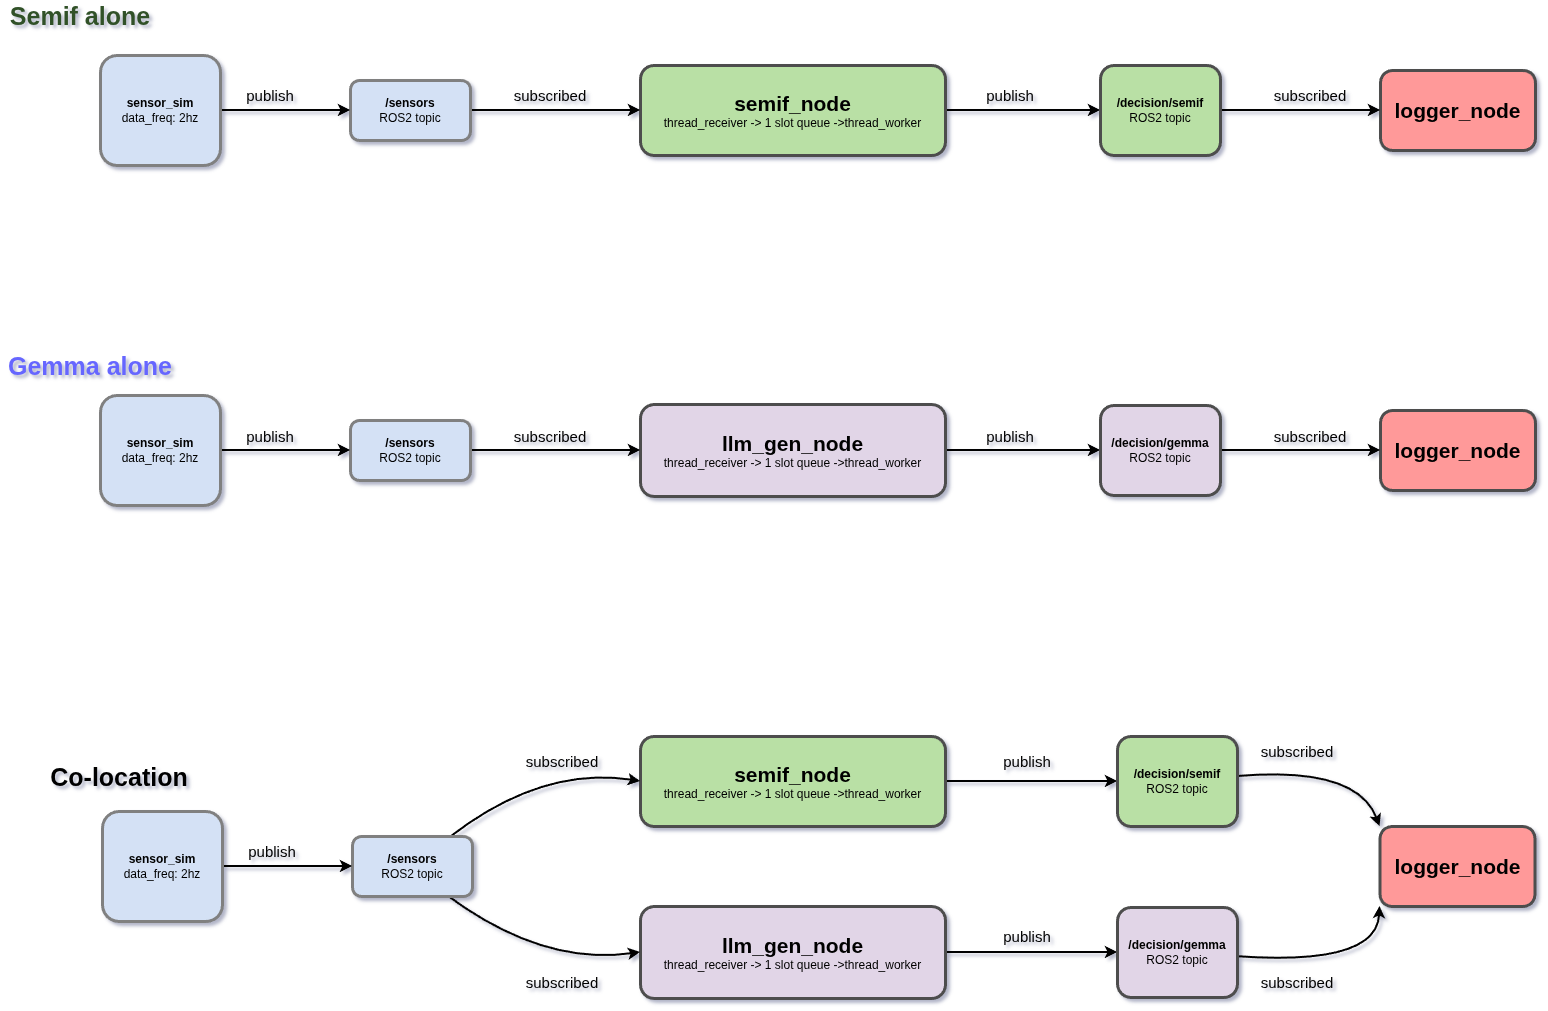
\includegraphics[width=0.97\columnwidth]{plots/markdown/0_infrastruttura/rtsia.drawio.png}
\caption{Architettura ROS e collegamenti tra sensori simulati, modelli e logger.}\label{fig:ros}
\end{figure}

\FloatBarrier
\subsection{Formato dei messaggi e richieste}
Il messaggio del sensore contiene il numero di sequenza, l'istante di generazione, l'azione attesa e una riga strutturata con stato, domanda e alternative. Il Listato~\ref{lst:sensor} ne illustra la struttura; le stringhe descrittive rappresentano segnaposto per i valori generati durante l'esecuzione. I testi delle alternative sono espressi in inglese, secondo il protocollo di interazione con i modelli.
\lstinputlisting[caption={Struttura del messaggio del sensore.},label={lst:sensor}]{Data/sensorsMsg.json}
SemIf riceve soltanto il campo \code{row} del messaggio, contenente \code{id}, \code{state}, \code{question} e \code{options}. Tale payload è riportato nel Listato~\ref{lst:semif}. Per Gemma, il nodo prepara la richiesta del Listato~\ref{lst:gemma}, con temperatura nulla, limite di 32 token e schema JSON che vincola l'azione alle tre alternative. Il vincolo sintattico non garantisce la correttezza semantica della decisione.
\lstinputlisting[caption={Payload strutturato inviato a SemIf.},label={lst:semif}]{Data/semifPayload.json}
\lstinputlisting[caption={Richiesta al server llama.cpp.},label={lst:gemma}]{Data/gemmaRequest.json}
I messaggi di risposta includono gli istanti di generazione, ingresso e uscita, l'azione prodotta, quella attesa e le statistiche di inferenza. Il campo \code{dropped} registra il numero di messaggi scartati.
\lstinputlisting[caption={Struttura della risposta dei nodi decisionali.},label={lst:decision}]{Data/decisionMsg.json}
\FloatBarrier
\subsection{Metriche e piano di confronto}
La latenza end-to-end, espressa in millisecondi, è definita come
\begin{equation}
L_{\mathrm{e2e}}=\frac{t_{\mathrm{out,ns}}-t_{\mathrm{gen,ns}}}{10^6}.
\end{equation}
Per distinguere l'attesa precedente all'invocazione dall'elaborazione del modello, si considera inoltre l'intervallo
\begin{equation}
L_{\mathrm{inf}}=\frac{t_{\mathrm{out,ns}}-t_{\mathrm{in,ns}}}{10^6}.
\end{equation}
Quest'ultimo può includere costi di invocazione e comunicazione; non rappresenta necessariamente il solo tempo dei kernel GPU. L'accuratezza confronta l'azione prodotta con quella attesa. Sono inoltre analizzate la composizione prefill/decode, le latenze di coda e la variabilità temporale. Il confronto considera sia la variabilità assoluta, espressa dal jitter, sia quella relativa, espressa dal coefficiente di variazione.
La Tabella~\ref{tab:blocks} organizza i cinque blocchi sperimentali, B1--B5. I piani successivi riportano sistema, stressore, livello configurato, modalità di isolamento, ripetizioni, durata della singola esecuzione e frequenza nominale dei sensori. Il campo livello indica l'intensità configurata del carico e non coincide necessariamente con il numero di worker effettivamente attivi.

\begin{table}[!htbp]
\centering
\caption{Blocchi sperimentali e fattori variati.}\label{tab:blocks}
\footnotesize

\begin{tabularx}{\columnwidth}{l >{\raggedright\arraybackslash}X >{\raggedright\arraybackslash}X}
\toprule
Blocco & Domanda & Parametri variati \\
\midrule
B1 Baseline & Come si comportano i due modelli quando eseguono singolarmente sul sistema e non vi è isolamento delle risorse & nessun parametro \\
B2 Co-locazione & Cosa succede quando i due modelli quando eseguono in contemporanea, o più in generale cosa accade quando i modelli girano in parallelo ad un carico sulla GPU & Uno o due modelli attivi \\
B3 Interferenze & Come degradano le prestazioni dei modelli quando sono presenti altri tipi di workload, sulla cpu, sulla memoria, o real time & Tipo di stress \\
B4 Isolamento & Come migliorano le prestazioni in presenza di altri workload, sfruttando le tecniche di isolamento & Tipo di stress e tecnica di isolamento \\
B5 Isolamento singolo & Come migliorano le prestazioni dei singoli modelli in colocation, applicando l’isolamento solo ad un modello alla volta & Tipo di stress, modello isolato \\
\bottomrule
\end{tabularx}
\end{table}

\FloatBarrier
\section{B1. Baseline}\label{sec:b1}

\FloatBarrier
\subsection{Piano sperimentale}
B1 determina il comportamento di riferimento dei modelli eseguiti singolarmente, in assenza di carichi concorrenti e di isolamento. Il piano prevede cinque ripetizioni per modello, con durata di 180 s per SemIf e 600 s per Gemma (Tabella~\ref{tab:b1}).

\begin{table}[!htbp]
\centering
\caption{Piano sperimentale B1: esecuzione individuale senza isolamento.}\label{tab:b1}
\scriptsize
\setlength{\tabcolsep}{2pt}
\begin{tabular}{lllllll}
\toprule
Sistema & Carico & Liv. & Isolamento & Rep. & $t$ (s) & $f$ (Hz) \\
\midrule
semif & none & 0 & none & 5 & 180 & 2 \\
gemma & none & 0 & none & 5 & 600 & 2 \\
\bottomrule
\end{tabular}
\end{table}

\FloatBarrier
\subsection{Latenza end-to-end e stabilità}
I boxplot di Fig.~\ref{fig:b1e2e} mostrano ordini di grandezza differenti: SemIf opera nell'intervallo delle centinaia di millisecondi, mentre Gemma richiede migliaia di millisecondi. SemIf presenta una dispersione assoluta contenuta attorno alla mediana. Per Gemma si osservano scostamenti dell'ordine di 500 ms e valori anomali prossimi a 9 s. Le latenze di coda in Fig.~\ref{fig:b1tail} confermano la maggiore variabilità assoluta di Gemma.

\begin{figure}[!htbp]
\centering
\includegraphics[width=0.97\columnwidth]{plots/markdown/b1_baseline/boxplot_latenza_e2e_singoli.png}
\caption{B1: distribuzioni della latenza end-to-end dei modelli eseguiti singolarmente.}\label{fig:b1e2e}
\end{figure}

\begin{figure}[!htbp]
\centering
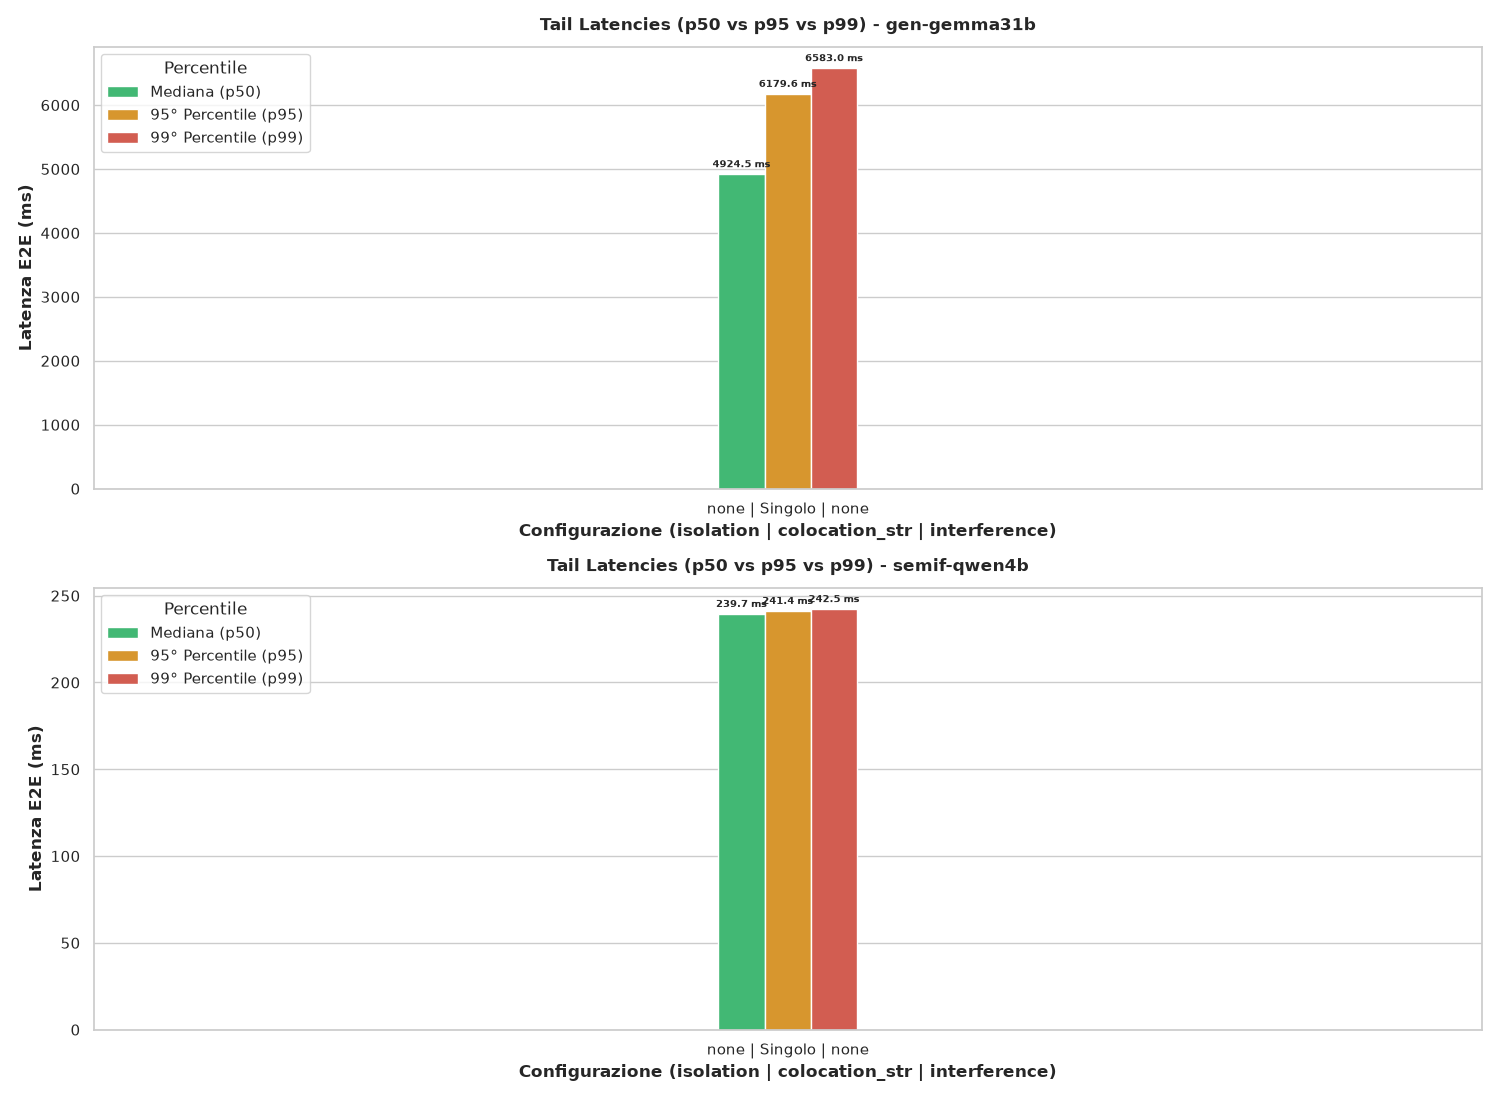
\includegraphics[width=0.97\columnwidth]{plots/markdown/b1_baseline/tail_latencies.png}
\caption{B1: confronto delle latenze di coda.}\label{fig:b1tail}
\end{figure}

\FloatBarrier
\subsection{Composizione del tempo di elaborazione}
La Fig.~\ref{fig:b1phases} evidenzia il costo della fase di decode di Gemma. Anche limitando il confronto alla fase di prefill, SemIf presenta tempi inferiori. Il tempo di inferenza di SemIf a riposo è pari a circa 238 ms.

\begin{figure}[!htbp]
\centering
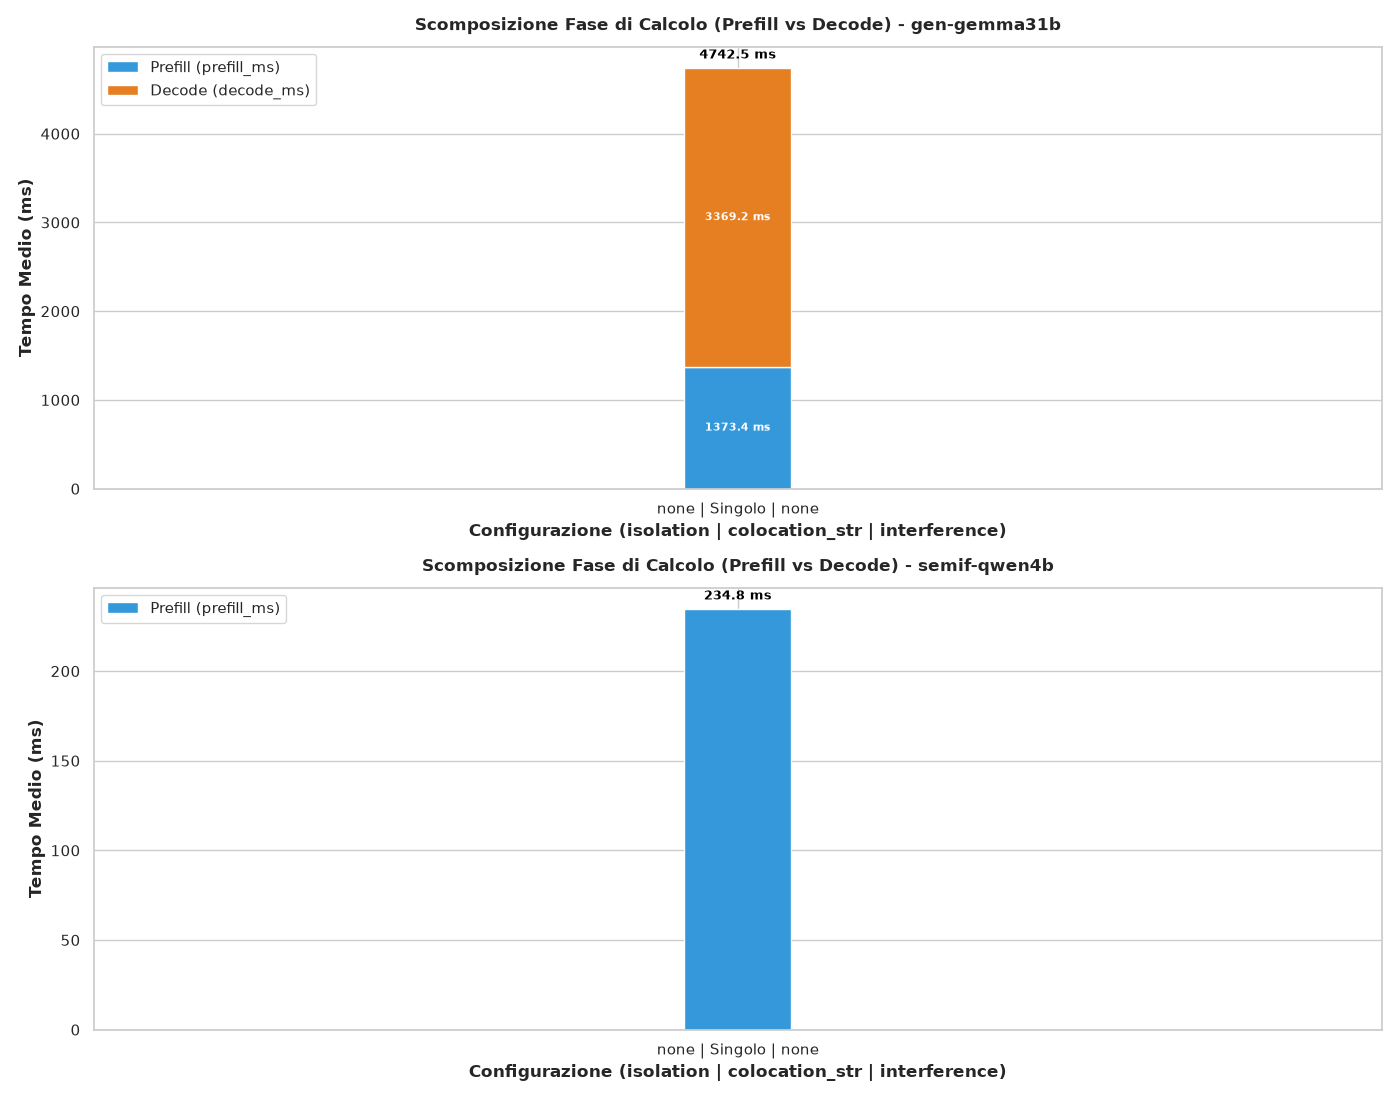
\includegraphics[width=0.97\columnwidth]{plots/markdown/b1_baseline/Prefill_decode.png}
\caption{B1: composizione dei tempi di elaborazione in prefill e decode.}\label{fig:b1phases}
\end{figure}

\FloatBarrier
\subsection{Accuratezza}
Il vantaggio temporale non coincide con una superiorità nell'accuratezza: la Fig.~\ref{fig:b1accuracy} documenta casi in cui SemIf è meno accurato di Gemma. Il confronto richiede pertanto di valutare congiuntamente correttezza e tempestività della decisione.

\begin{figure}[!htbp]
\centering
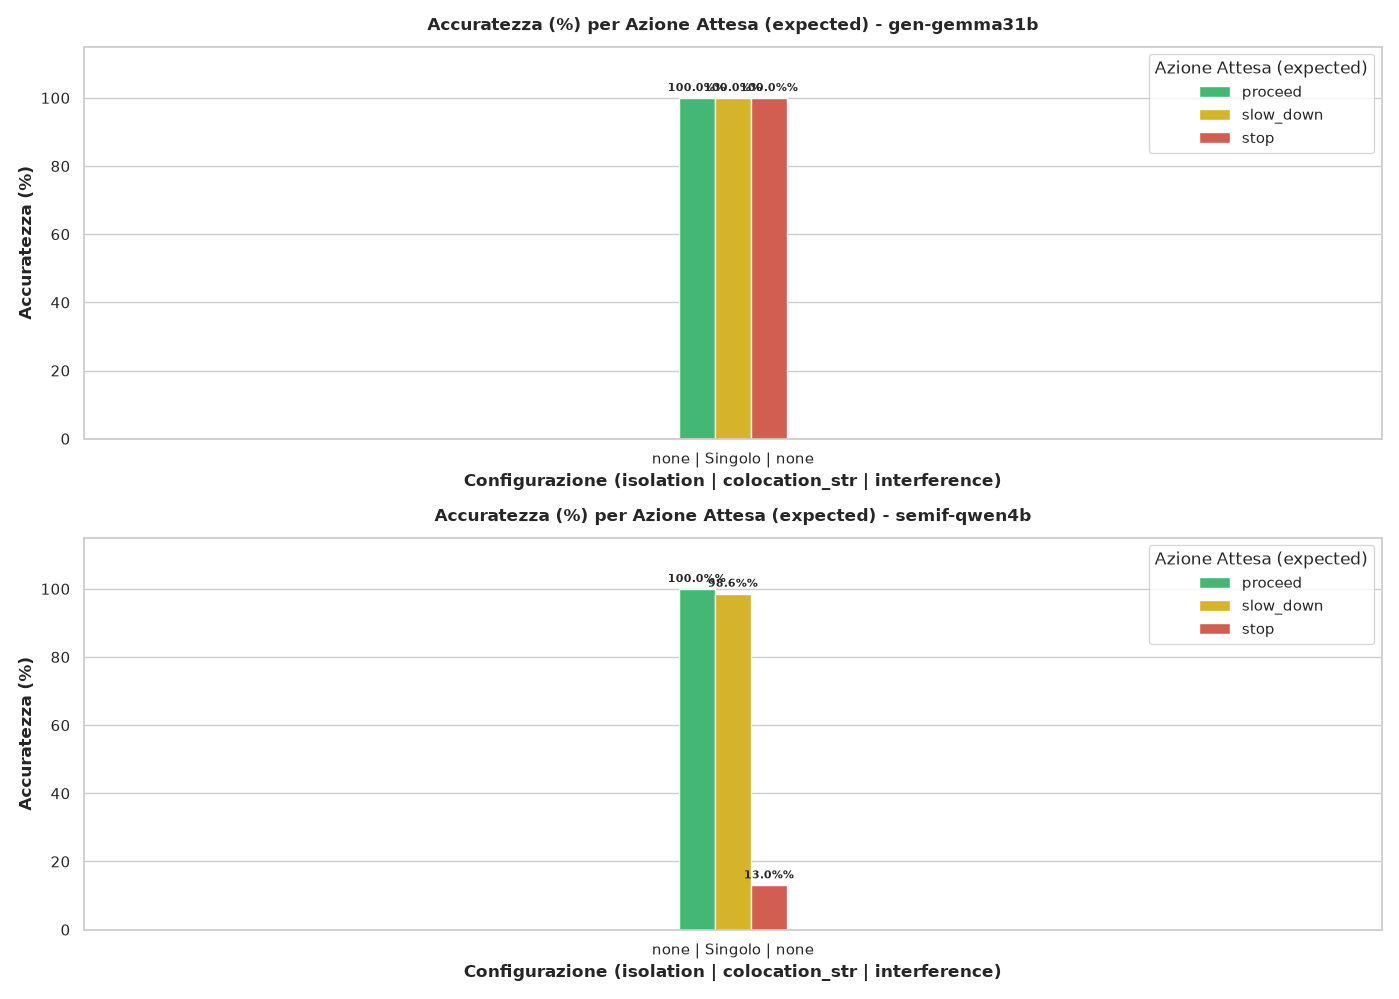
\includegraphics[width=0.97\columnwidth]{plots/markdown/b1_baseline/accuracy.png}
\caption{B1: accuratezza delle decisioni rispetto all’azione attesa.}\label{fig:b1accuracy}
\end{figure}

\FloatBarrier
\section{B2. Co-locazione}\label{sec:b2}

\FloatBarrier
\subsection{Piano sperimentale}
B2 valuta l'interferenza reciproca quando i due modelli condividono la GPU. SemIf e Gemma elaborano simultaneamente i dati dei sensori, senza isolamento e senza stressori aggiuntivi. Sono previste cinque ripetizioni da 600 s, come riportato nella Tabella~\ref{tab:b2}.

\begin{table}[!htbp]
\centering
\caption{Piano sperimentale B2: co-locazione sulla GPU.}\label{tab:b2}
\scriptsize
\setlength{\tabcolsep}{2pt}
\begin{tabular}{lllllll}
\toprule
Sistema & Carico & Liv. & Isolamento & Rep. & $t$ (s) & $f$ (Hz) \\
\midrule
semif,gemma & none & 0 & none & 5 & 600 & 2 \\
\bottomrule
\end{tabular}
\end{table}

\FloatBarrier
\subsection{Ritardo end-to-end e inferenza}
Le Figg.~\ref{fig:b2e2e} e~\ref{fig:b2comparison} mostrano un incremento della latenza rispetto all'esecuzione individuale. SemIf risulta il modello maggiormente penalizzato in termini relativi. Una possibile interpretazione è la prolungata occupazione della GPU da parte di Gemma; tale ipotesi richiede una verifica mediante tracciamento dello scheduling dei kernel.
La Fig.~\ref{fig:b2inf} considera l'intervallo di inferenza, separandolo dall'attesa precedente all'invocazione. Il peggioramento anche di questa metrica indica che il degrado non riguarda soltanto l'accumulo delle richieste.

\begin{figure}[!htbp]
\centering
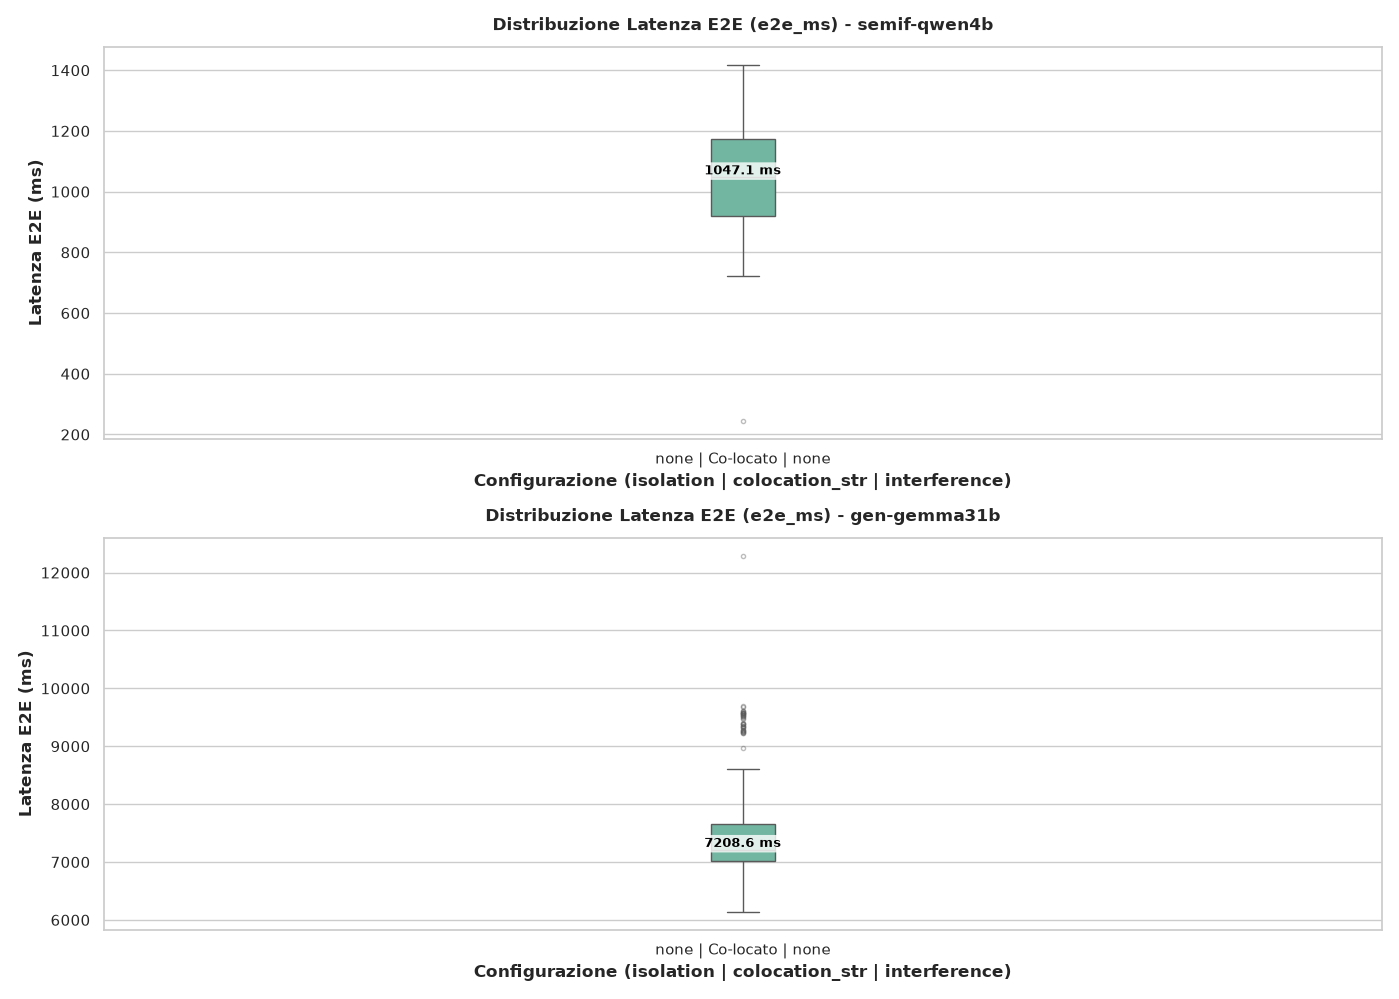
\includegraphics[width=0.97\columnwidth]{plots/markdown/b2_co_location/bp_latenzaE2E.png}
\caption{B2: latenza end-to-end durante l’esecuzione simultanea.}\label{fig:b2e2e}
\end{figure}

\begin{figure}[!htbp]
\centering
\includegraphics[width=0.97\columnwidth]{plots/markdown/b2_co_location/boxplot_latenza_e2e_singoli.png}
\caption{Distribuzioni della latenza end-to-end nell'esecuzione individuale, utilizzate come riferimento per B2.}\label{fig:b2comparison}
\end{figure}

\begin{figure}[!htbp]
\centering
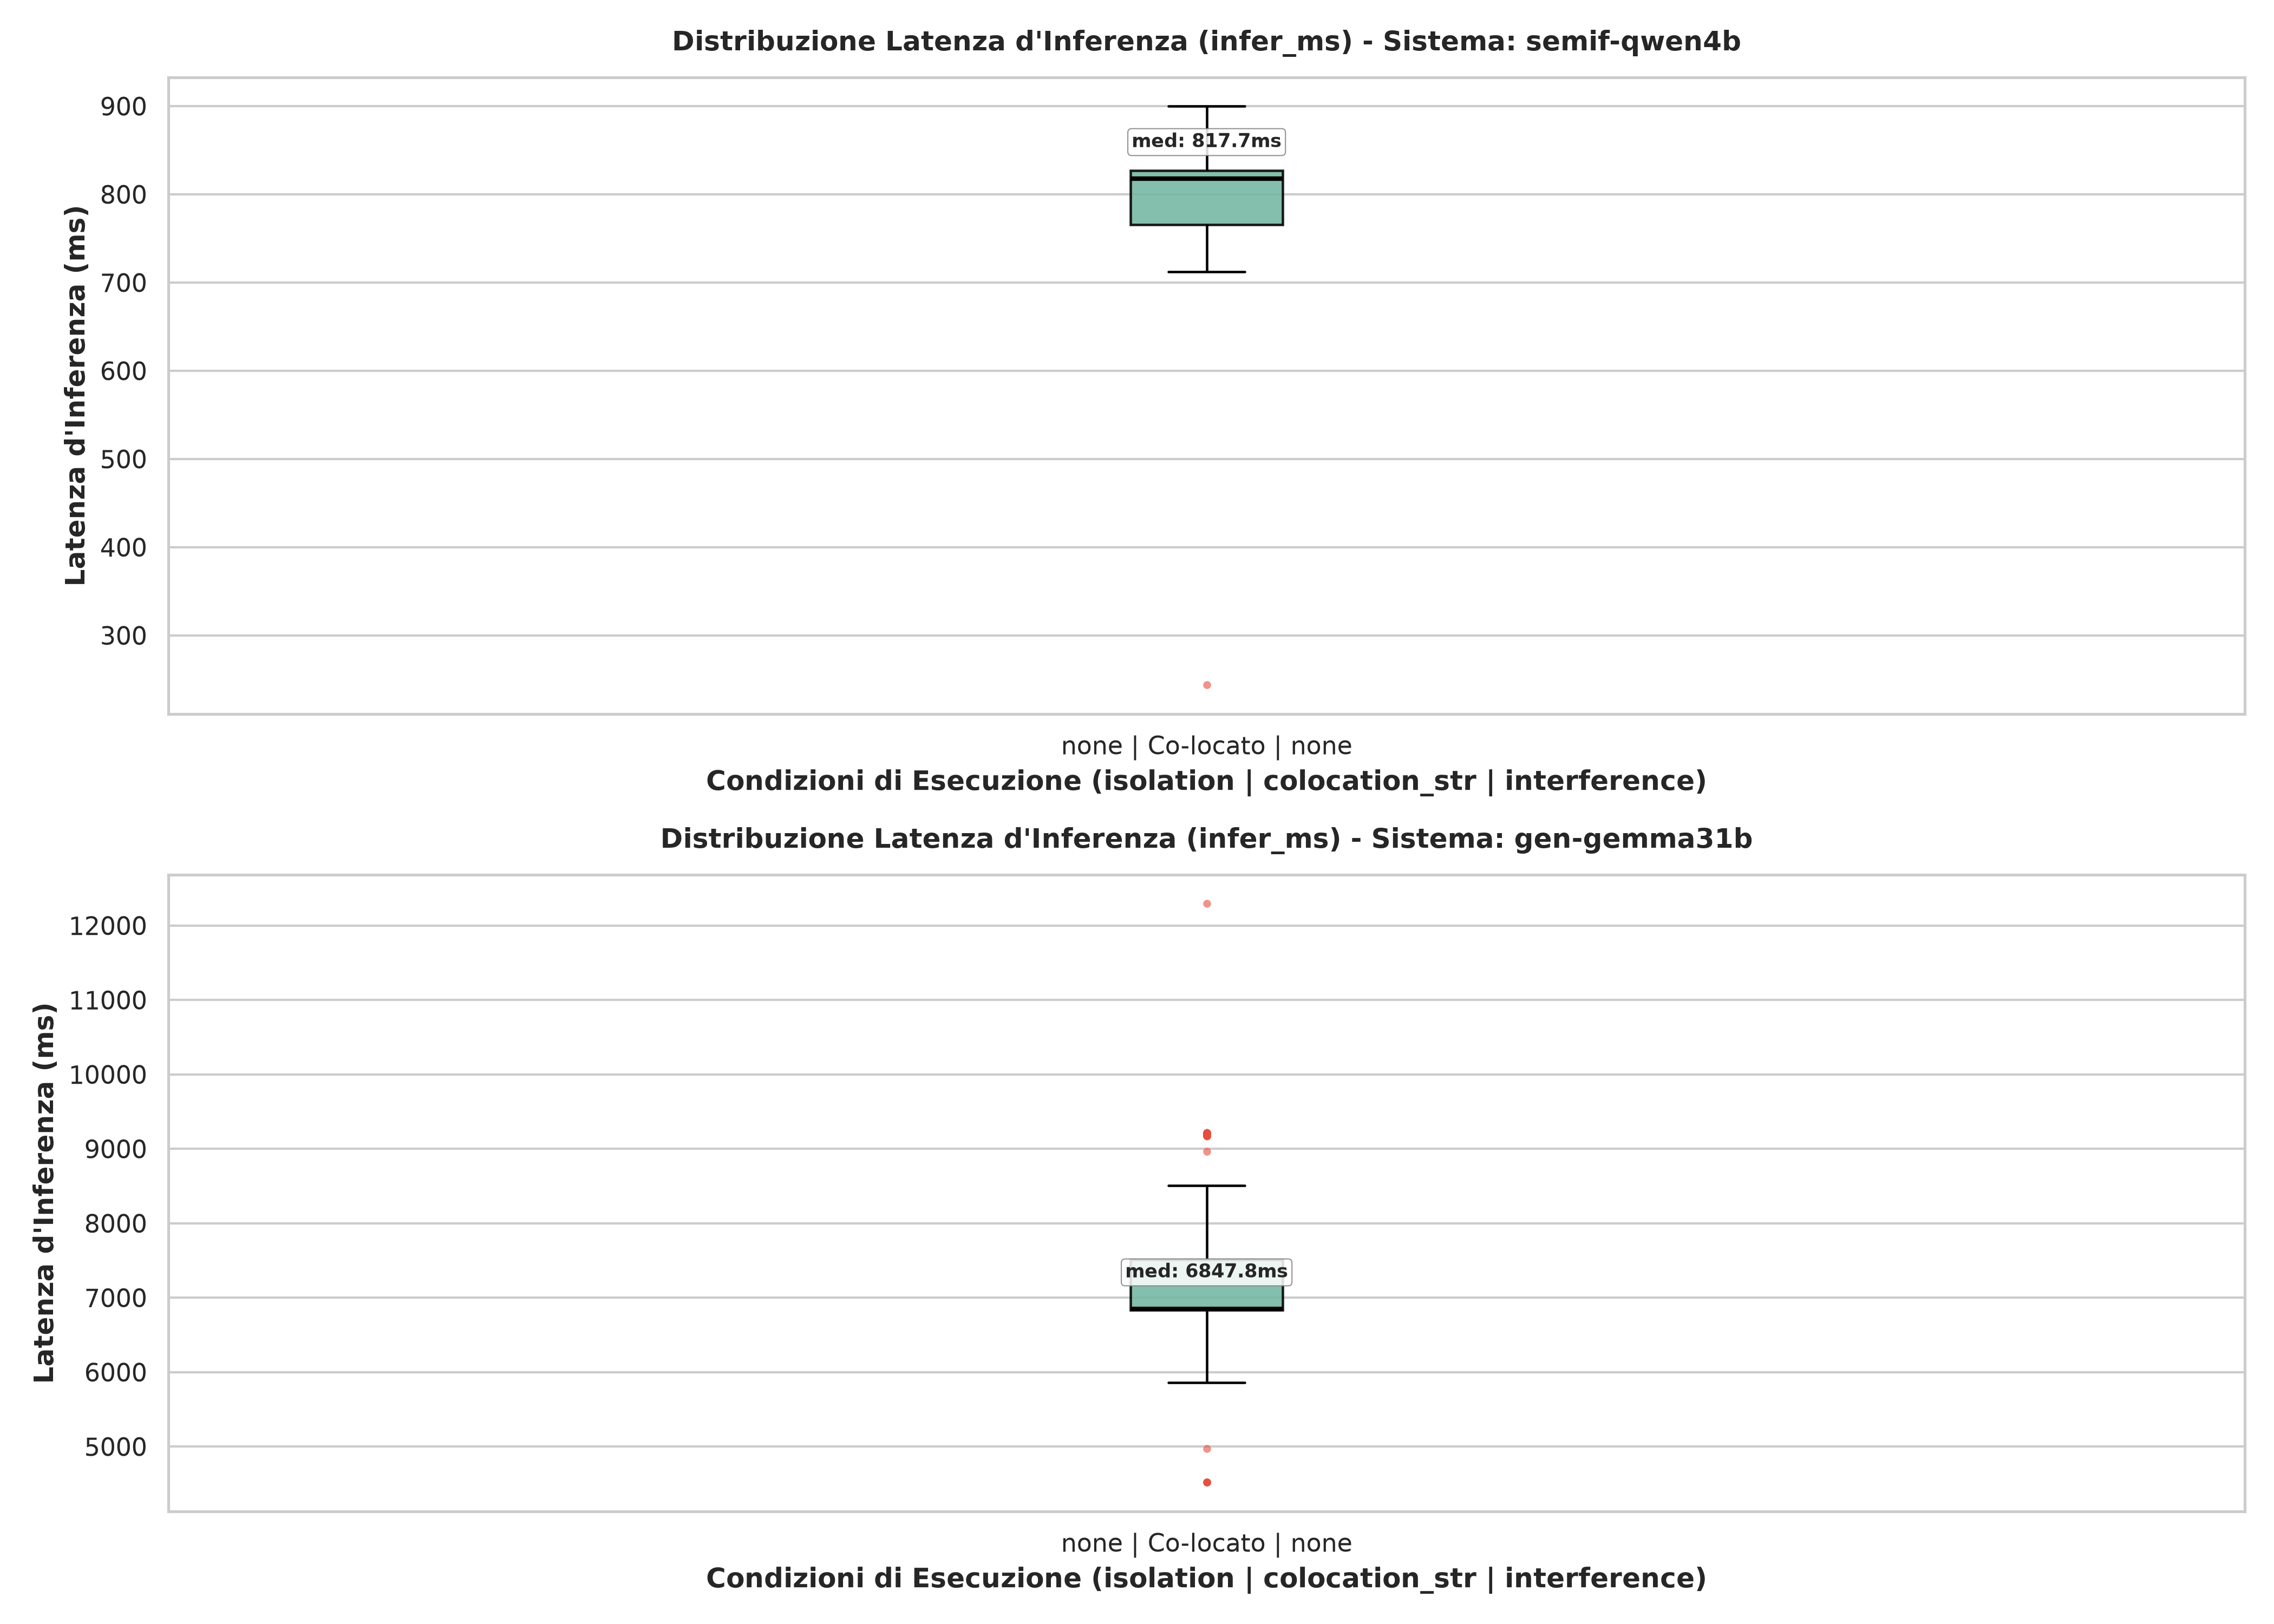
\includegraphics[width=0.97\columnwidth]{plots/markdown/b2_co_location/boxplot_infer_ms.png}
\caption{B2: distribuzioni della latenza di inferenza.}\label{fig:b2inf}
\end{figure}

\FloatBarrier
\subsection{Stabilità}
Nonostante il rallentamento, SemIf mantiene una variabilità assoluta inferiore. Il jitter è pari a 35,5 ms per SemIf e 780,5 ms per Gemma (Fig.~\ref{fig:b2jitter}).

\begin{figure}[!htbp]
\centering
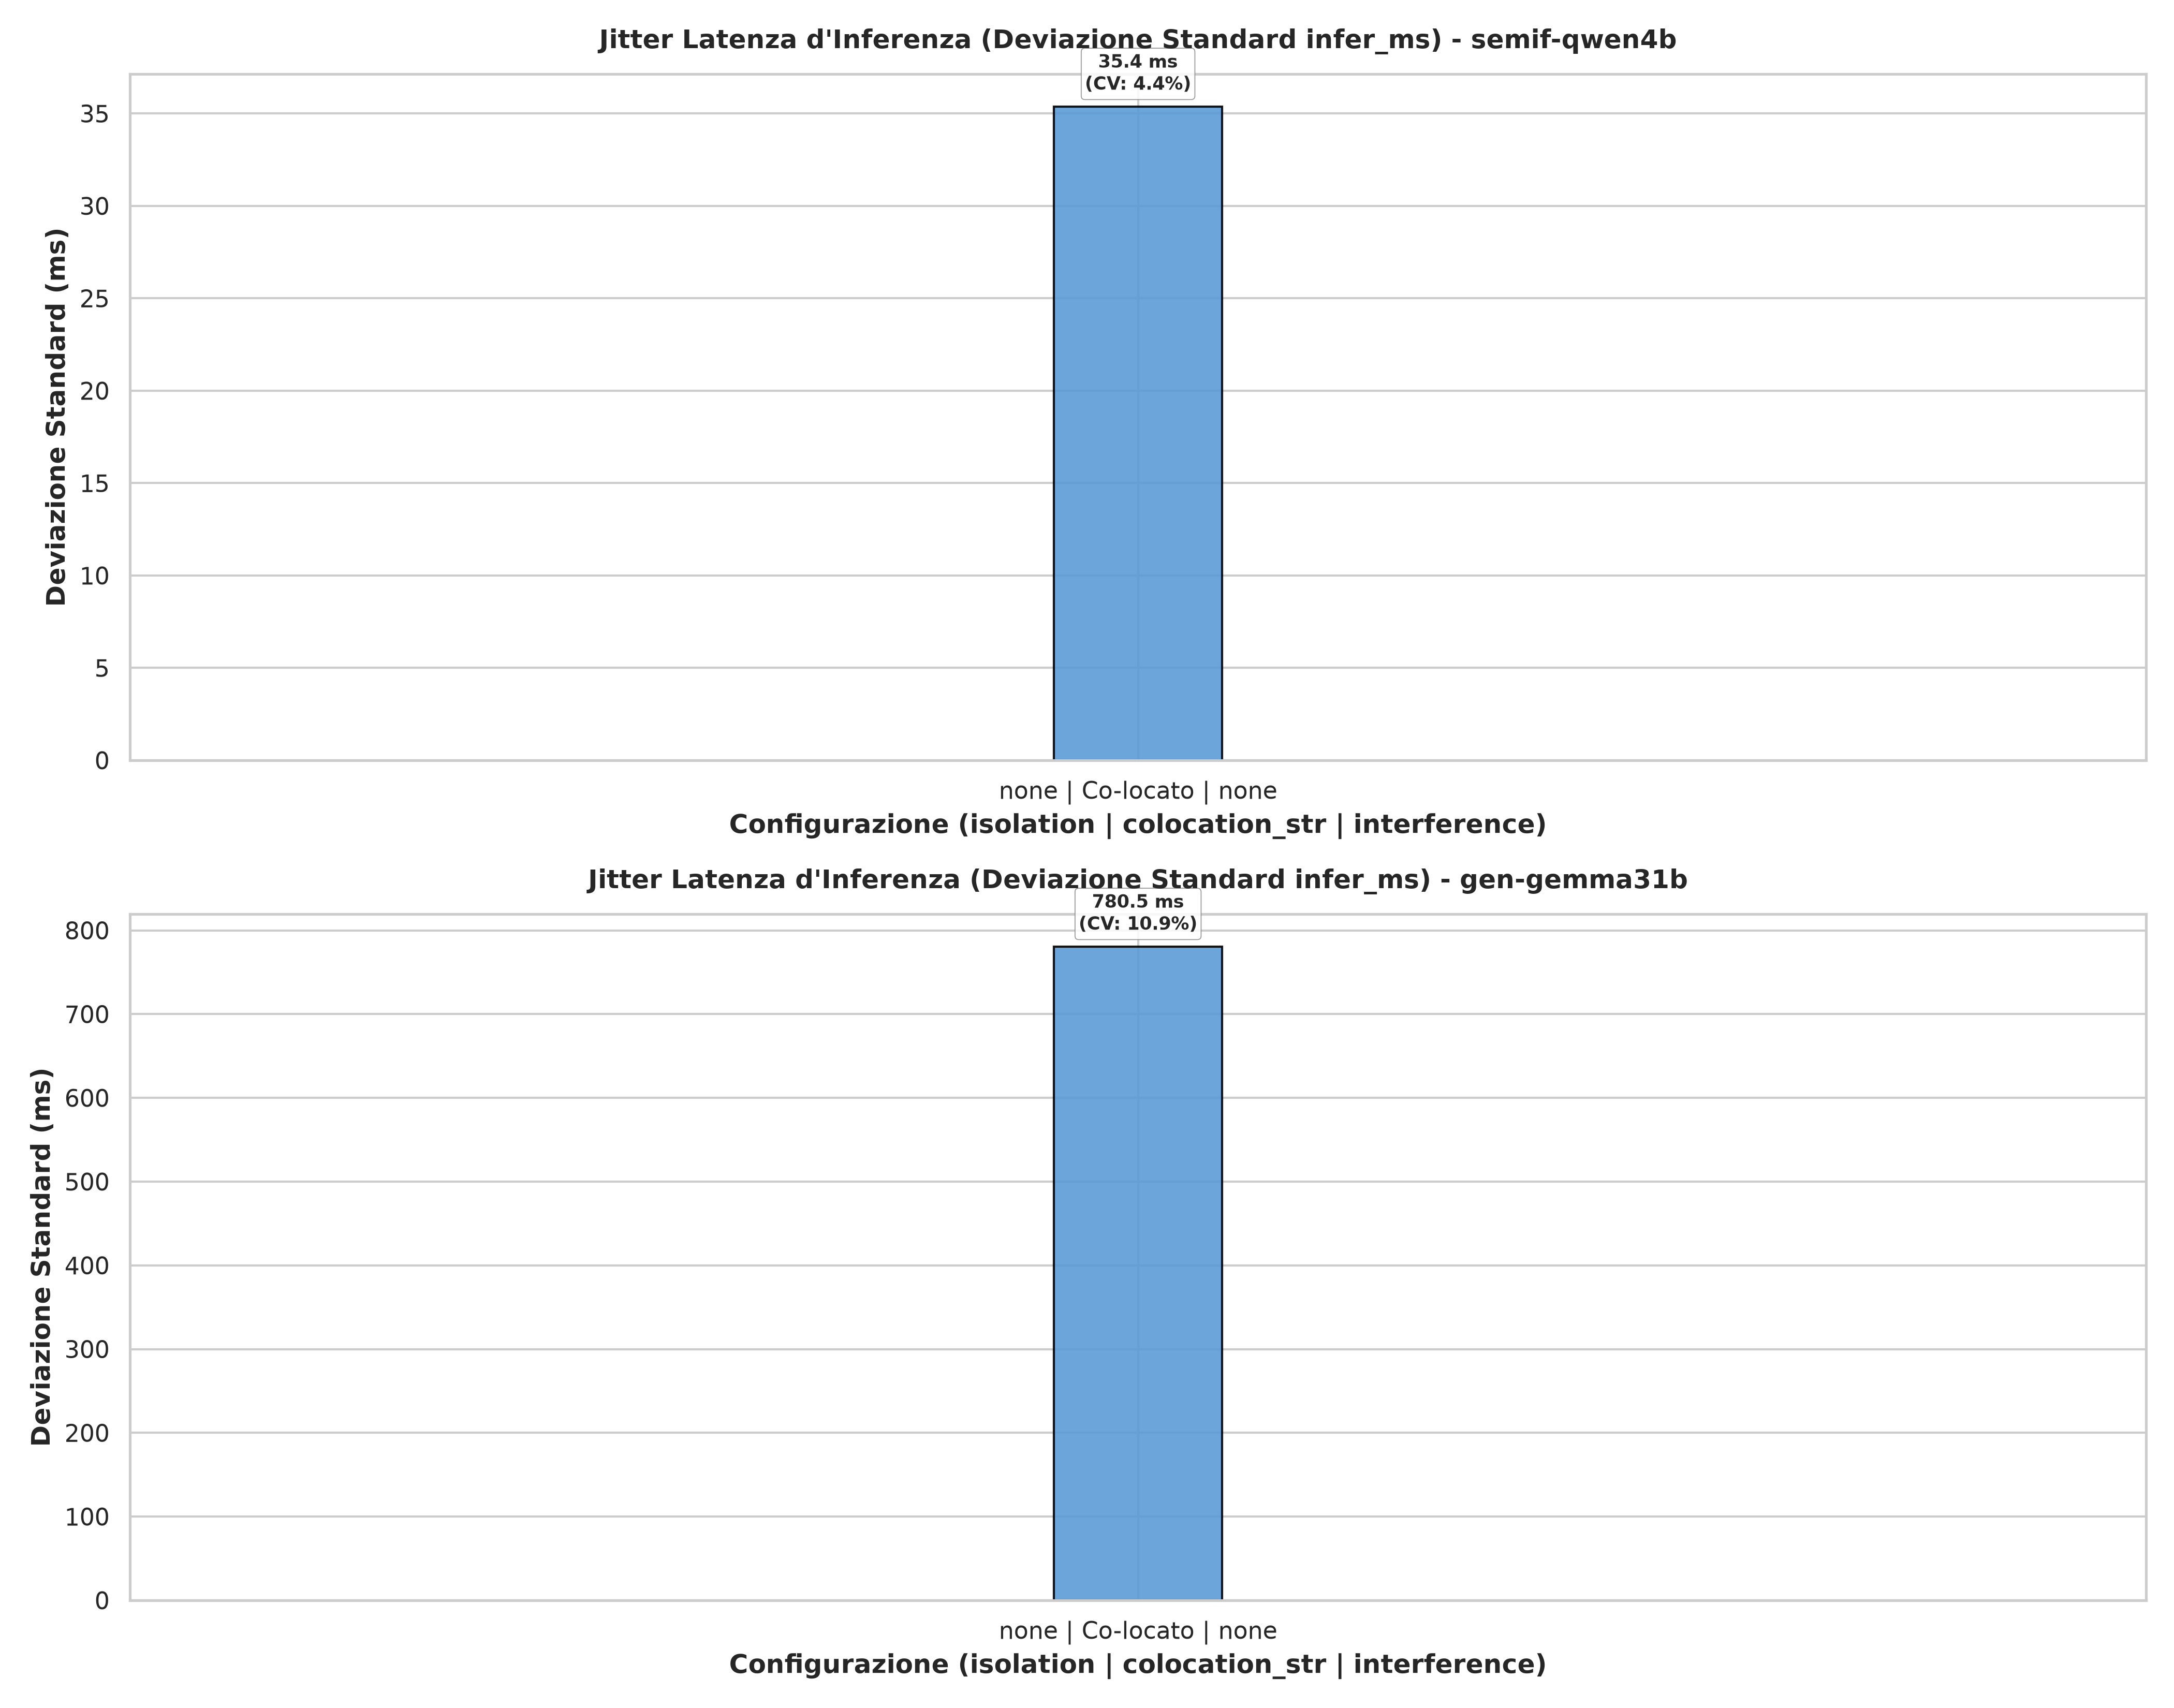
\includegraphics[width=0.97\columnwidth]{plots/markdown/b2_co_location/jitter_infer_ms.png}
\caption{B2: jitter e variabilità dei tempi di inferenza.}\label{fig:b2jitter}
\end{figure}

\FloatBarrier
\subsection{Fasi di elaborazione}
Le Figg.~\ref{fig:b2phases} e~\ref{fig:b2decode} indicano che, per Gemma, la fase maggiormente penalizzata è il decode, con un incremento di circa 1691,3 ms rispetto alla baseline.

\begin{figure}[!htbp]
\centering
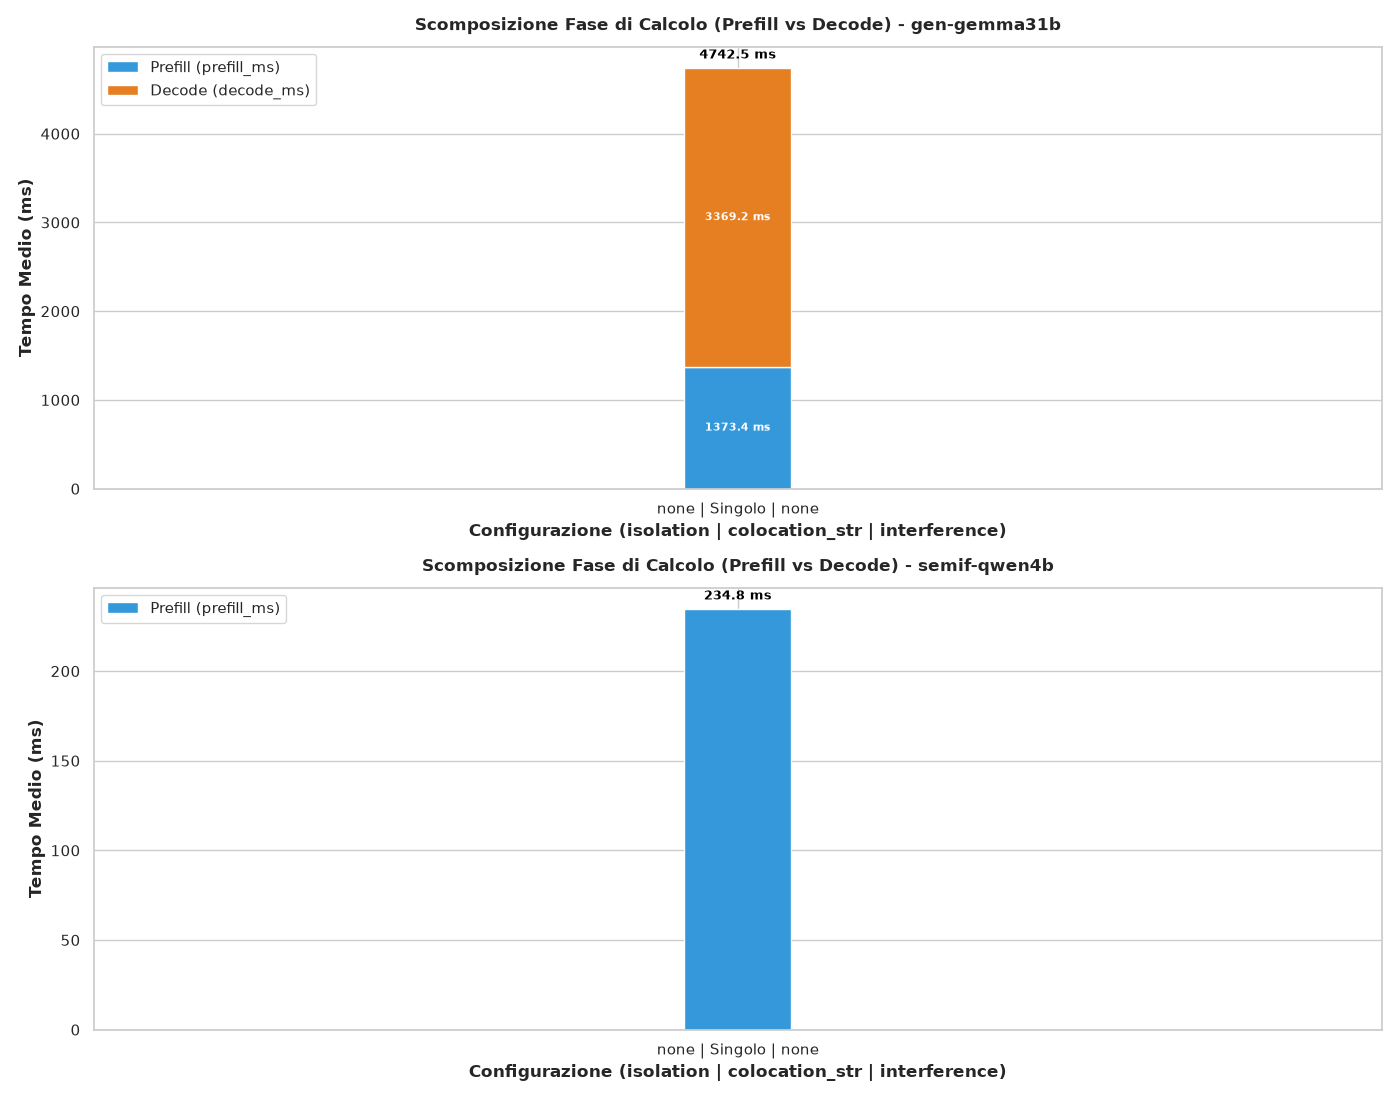
\includegraphics[width=0.97\columnwidth]{plots/markdown/b2_co_location/Prefill_decode.png}
\caption{Composizione dei tempi di prefill e decode nel confronto B2.}\label{fig:b2phases}
\end{figure}

\begin{figure}[!htbp]
\centering
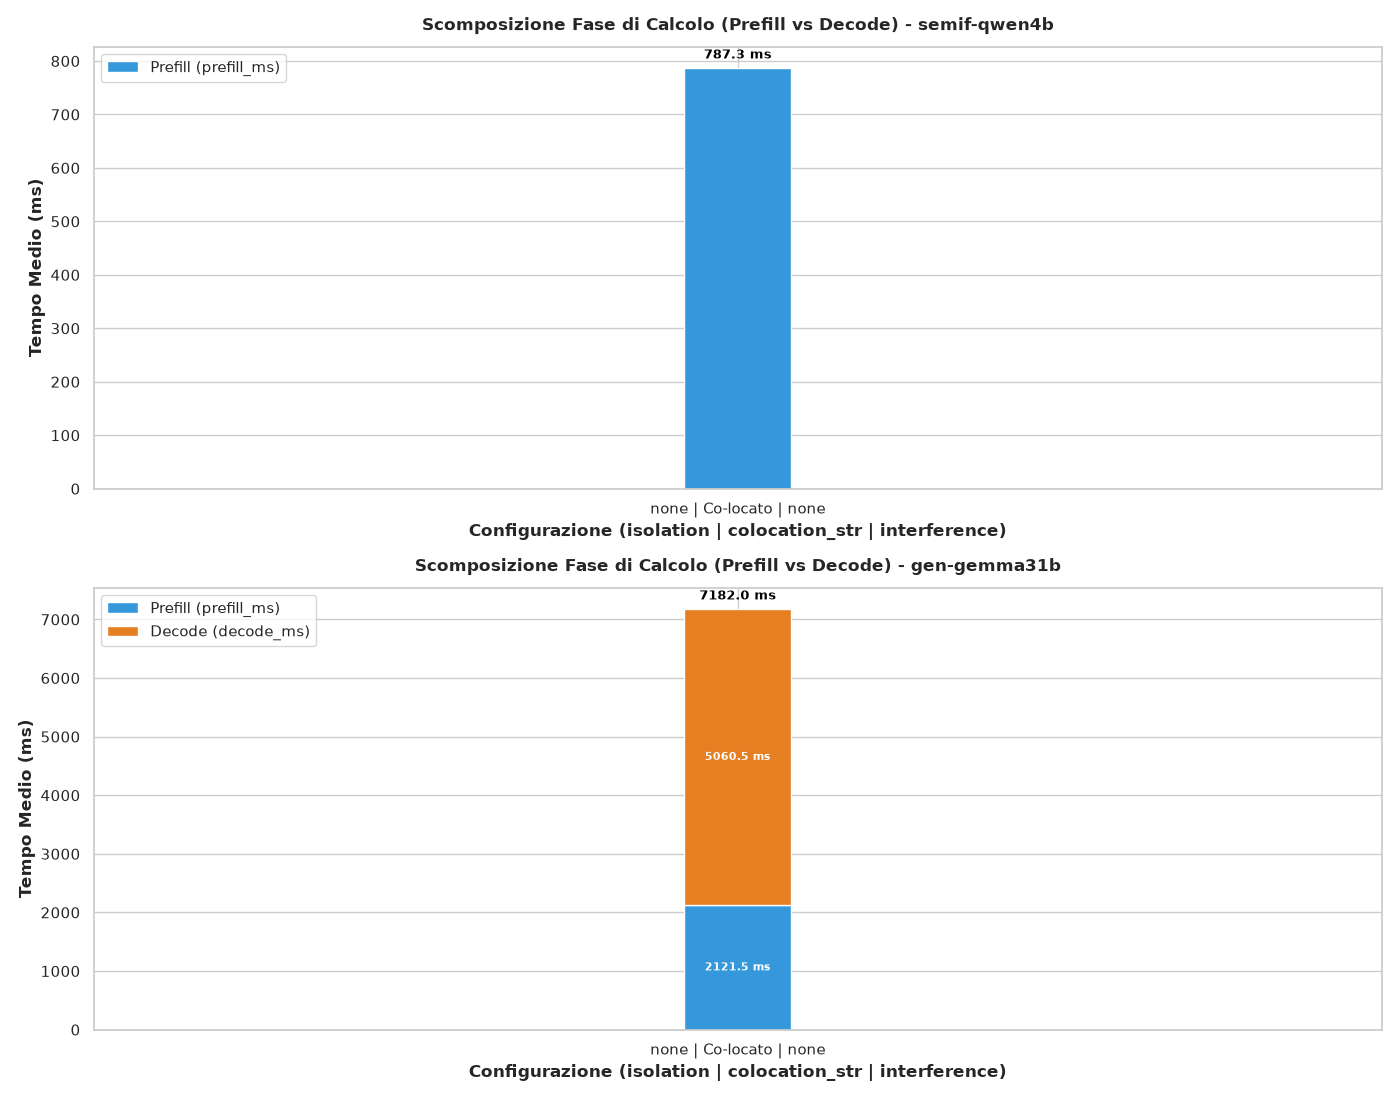
\includegraphics[width=0.97\columnwidth]{plots/markdown/b2_co_location/decodePrefill.png}
\caption{B2: confronto dei tempi di prefill e decode.}\label{fig:b2decode}
\end{figure}

\FloatBarrier
\section{B3. Interferenze}\label{sec:b3}

\FloatBarrier
\subsection{Piano sperimentale}
B3 introduce carichi concorrenti sulla CPU, sulla memoria e sulla cache, mantenendo disabilitato l'isolamento. Si utilizzano \code{stress-ng} per i carichi non real-time e \code{rt-app} per quelli real-time. Il piano di Tabella~\ref{tab:b3} prevede tre ripetizioni per configurazione, con durata di 180 s per SemIf e 300 s per Gemma.

\begin{table}[!htbp]
\centering
\caption{Piano sperimentale B3: interferenze senza isolamento.}\label{tab:b3}
\scriptsize
\setlength{\tabcolsep}{2pt}
\begin{tabular}{lllllll}
\toprule
Sistema & Carico & Liv. & Isolamento & Rep. & $t$ (s) & $f$ (Hz) \\
\midrule
semif & cpu\_matrix & 12 & none & 3 & 180 & 2 \\
semif & mem\_stream & 12 & none & 3 & 180 & 2 \\
semif & mem\_vm & 12 & none & 3 & 180 & 2 \\
semif & cache\_l1 & 12 & none & 3 & 180 & 2 \\
semif & sched\_switch & 12 & none & 3 & 180 & 2 \\
semif & rtapp\_other & 11 & none & 3 & 180 & 2 \\
semif & rtapp\_fifo60 & 11 & none & 3 & 180 & 2 \\
semif & rtapp\_burst60 & 11 & none & 3 & 180 & 2 \\
gemma & cpu\_matrix & 12 & none & 3 & 300 & 2 \\
gemma & mem\_stream & 12 & none & 3 & 300 & 2 \\
gemma & sched\_switch & 12 & none & 3 & 300 & 2 \\
gemma & mem\_vm & 12 & none & 3 & 300 & 2 \\
gemma & cache\_l1 & 12 & none & 3 & 300 & 2 \\
gemma & rtapp\_other & 11 & none & 3 & 300 & 2 \\
gemma & rtapp\_fifo60 & 11 & none & 3 & 300 & 2 \\
gemma & rtapp\_burst60 & 11 & none & 3 & 300 & 2 \\
\bottomrule
\end{tabular}
\end{table}

\FloatBarrier
\subsection{Degrado delle latenze e stabilità}
I carichi più penalizzanti risultano \code{sched_switch}, \code{mem_stream} e \code{mem_vm}, come illustrato nelle Figg.~\ref{fig:b3inf} e~\ref{fig:b3e2e}. Nei test descritti, i carichi real-time producono perturbazioni più contenute. L'effetto di \code{sched_switch} è coerente con un aumento delle interruzioni dell'esecuzione dei thread CPU che orchestrano l'inferenza sulla GPU.

\begin{figure}[!htbp]
\centering
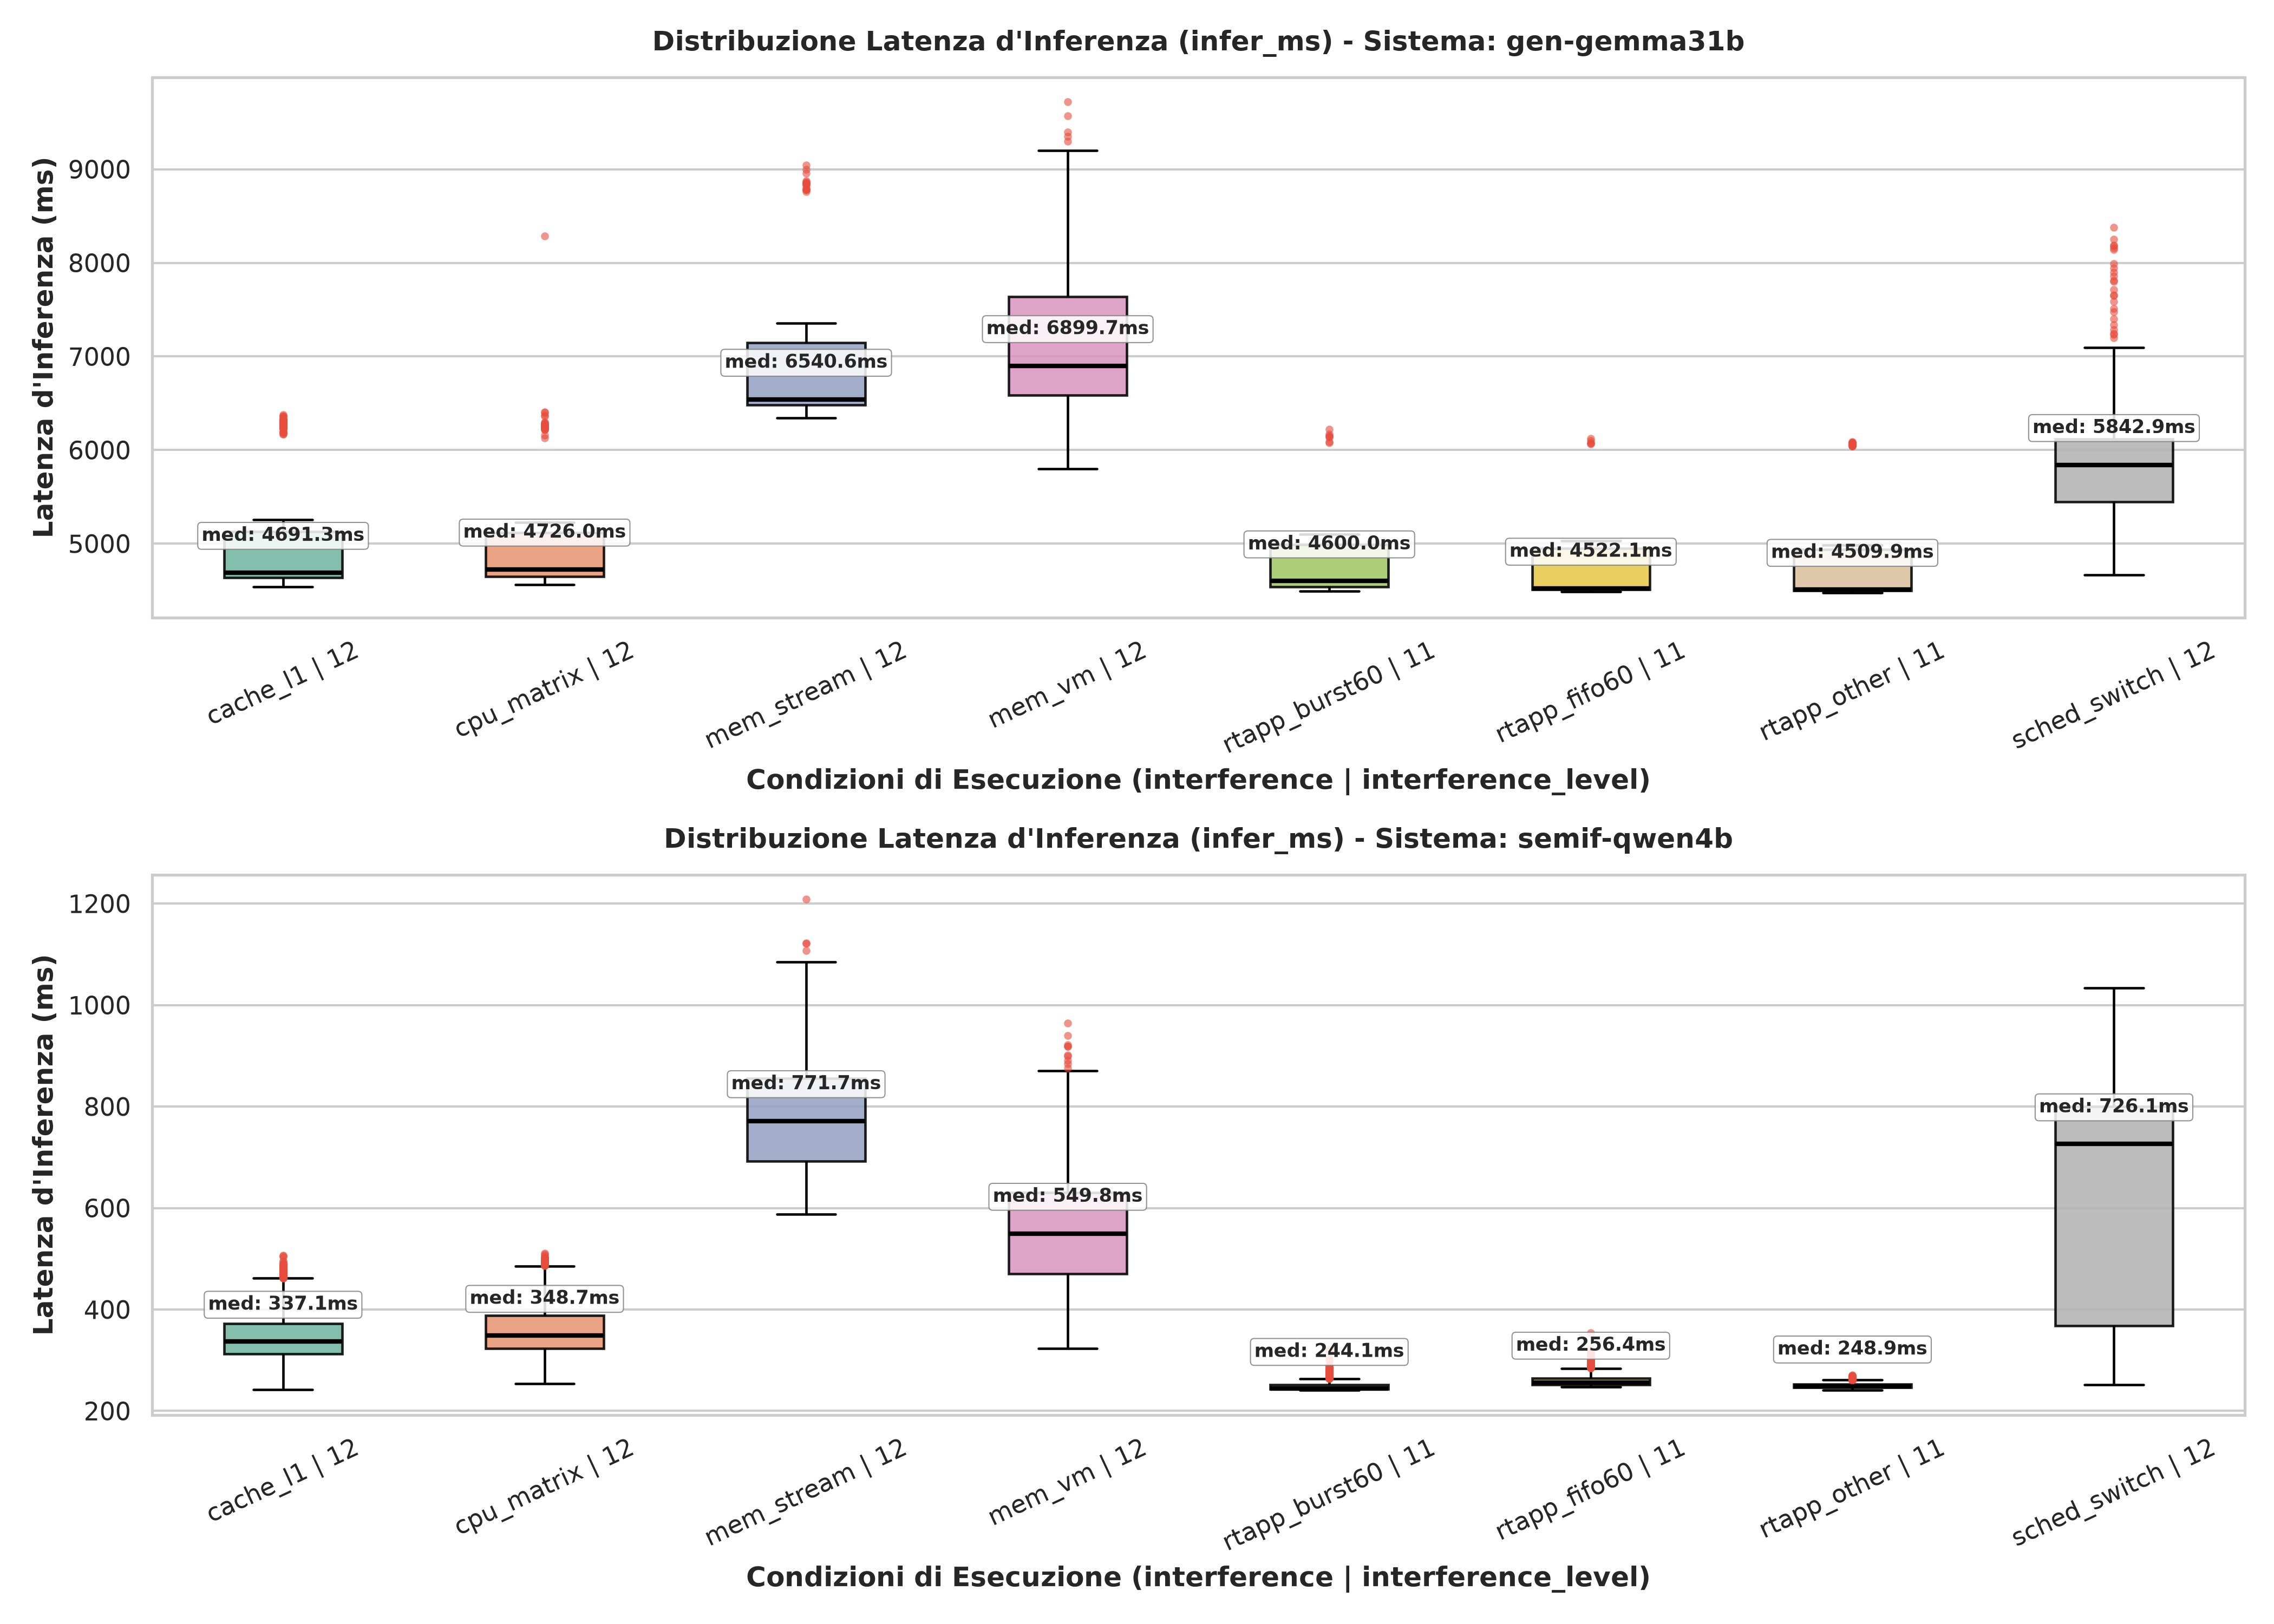
\includegraphics[width=0.97\columnwidth]{plots/markdown/b3_interference/boxplot_infer_ms.png}
\caption{B3: latenza di inferenza in presenza dei diversi carichi concorrenti.}\label{fig:b3inf}
\end{figure}

\begin{figure}[!htbp]
\centering
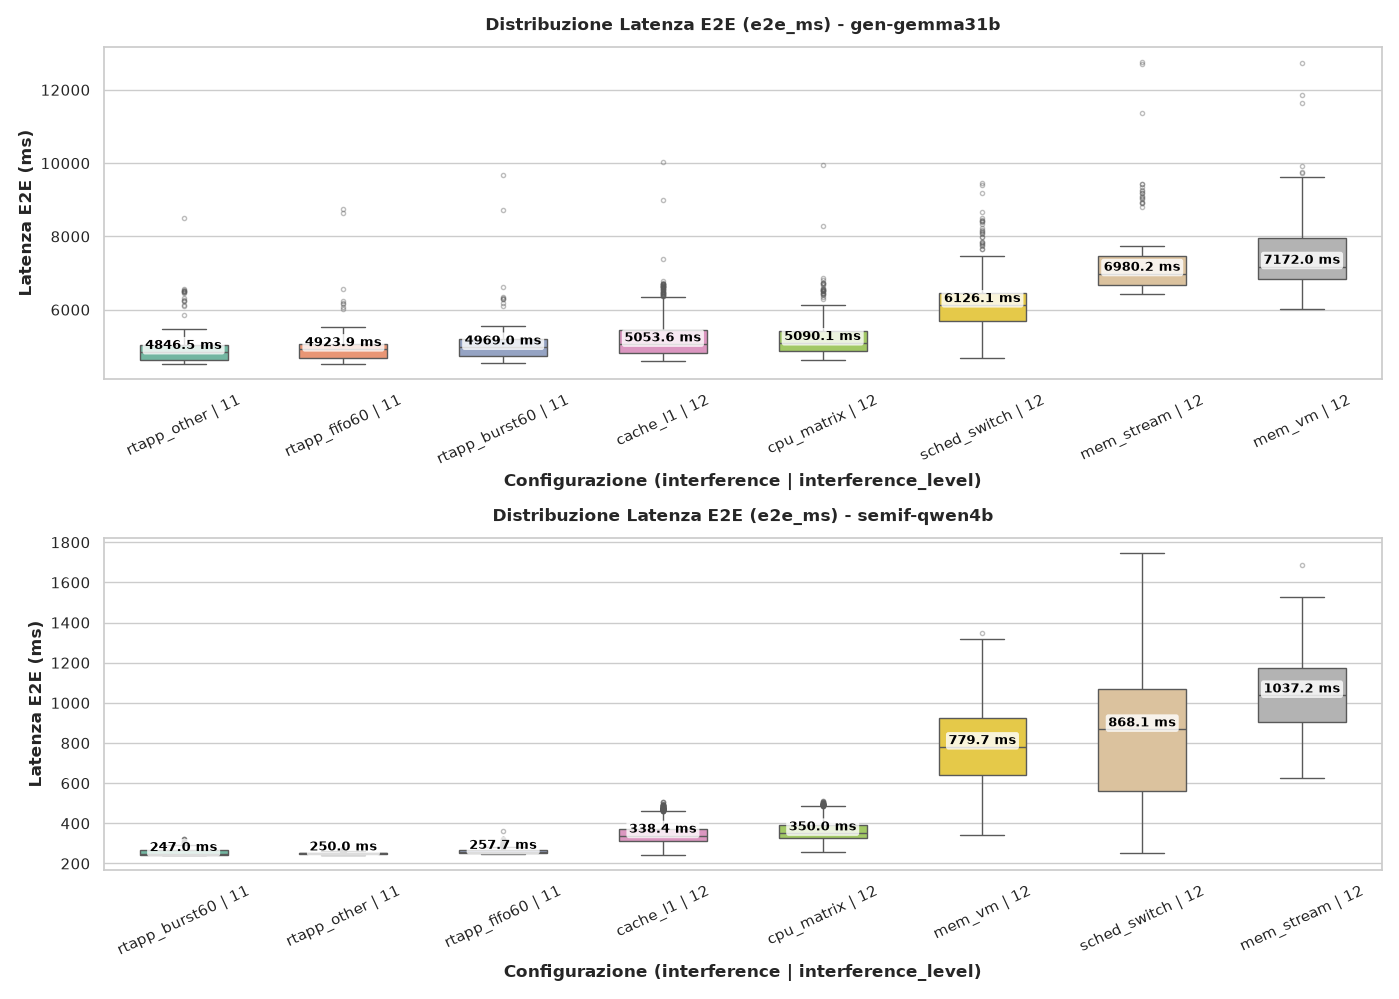
\includegraphics[width=0.97\columnwidth]{plots/markdown/b3_interference/boxplots_e2e.png}
\caption{B3: latenza end-to-end in presenza di interferenze.}\label{fig:b3e2e}
\end{figure}

\FloatBarrier
\subsection{Latenze di coda e stabilità}
Le latenze di coda raggiungono circa 12 s per Gemma e 1,4 s per SemIf (Fig.~\ref{fig:b3tail}); per Gemma si osservano anche casi superiori a 12 s. Tali massimi osservati non costituiscono limiti superiori garantiti. La Fig.~\ref{fig:b3jitter} mostra che SemIf conserva una minore variabilità assoluta. Un coefficiente di variazione inferiore per Gemma non implicherebbe necessariamente oscillazioni assolute inferiori, poiché tale indicatore normalizza la dispersione rispetto alla media.

\begin{figure}[!htbp]
\centering
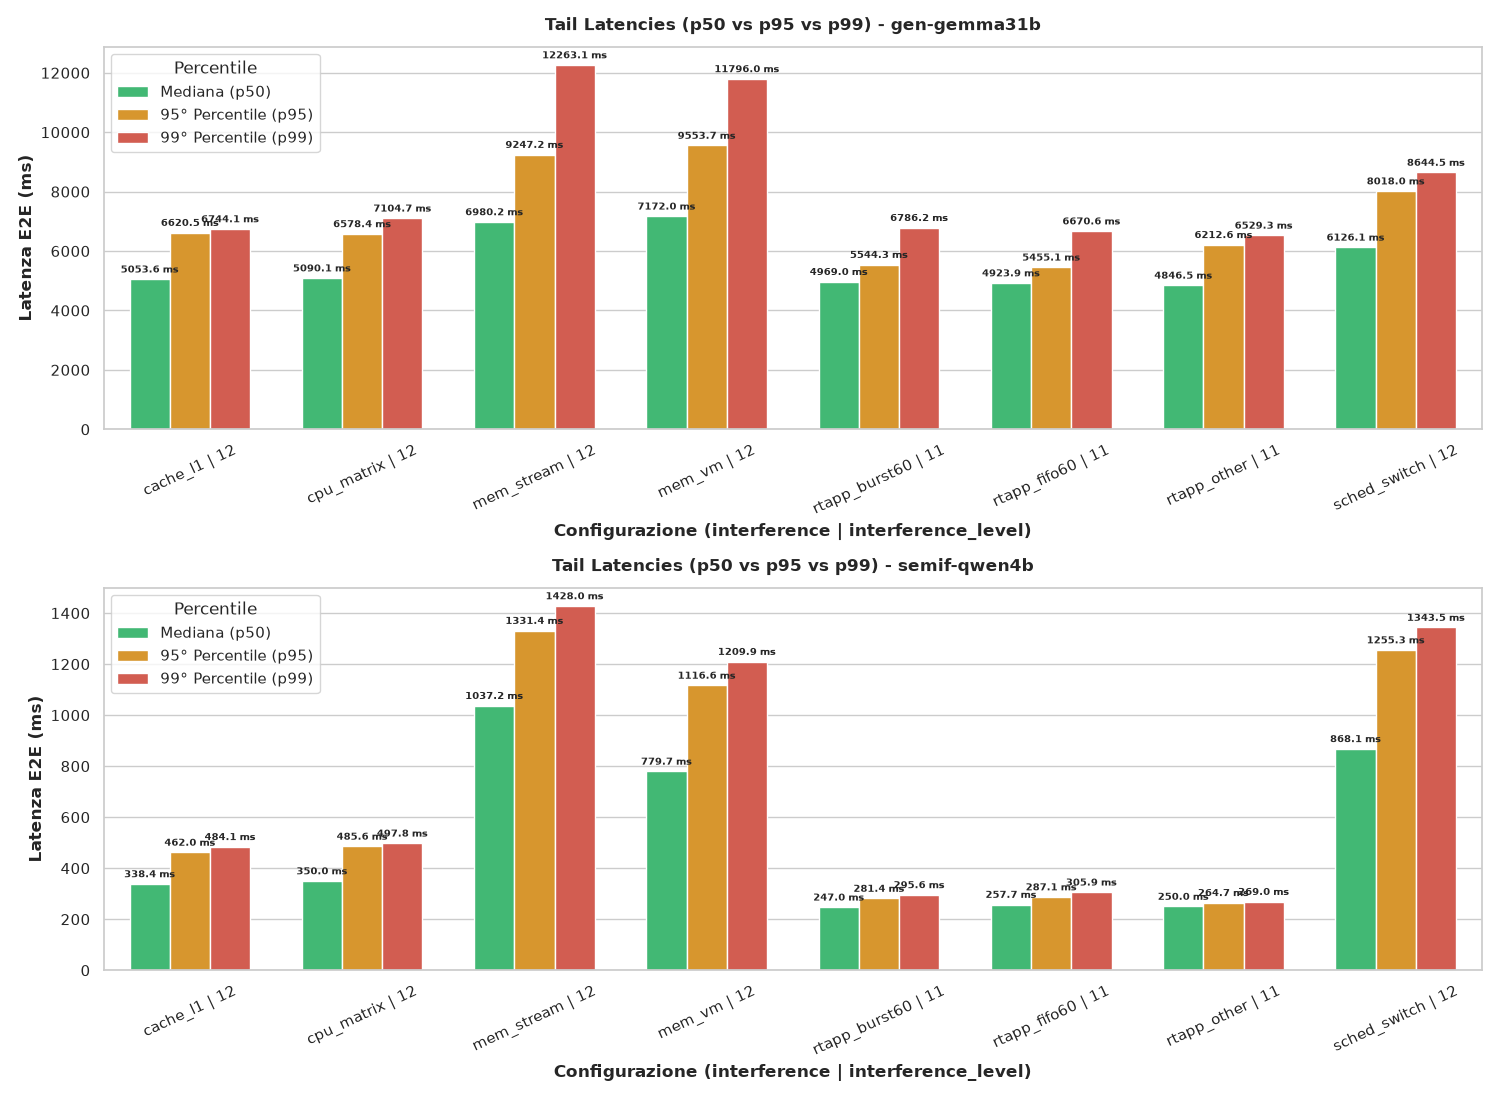
\includegraphics[width=0.97\columnwidth]{plots/markdown/b3_interference/tail_latencies.png}
\caption{B3: latenze di coda sotto interferenza.}\label{fig:b3tail}
\end{figure}

\begin{figure}[!htbp]
\centering
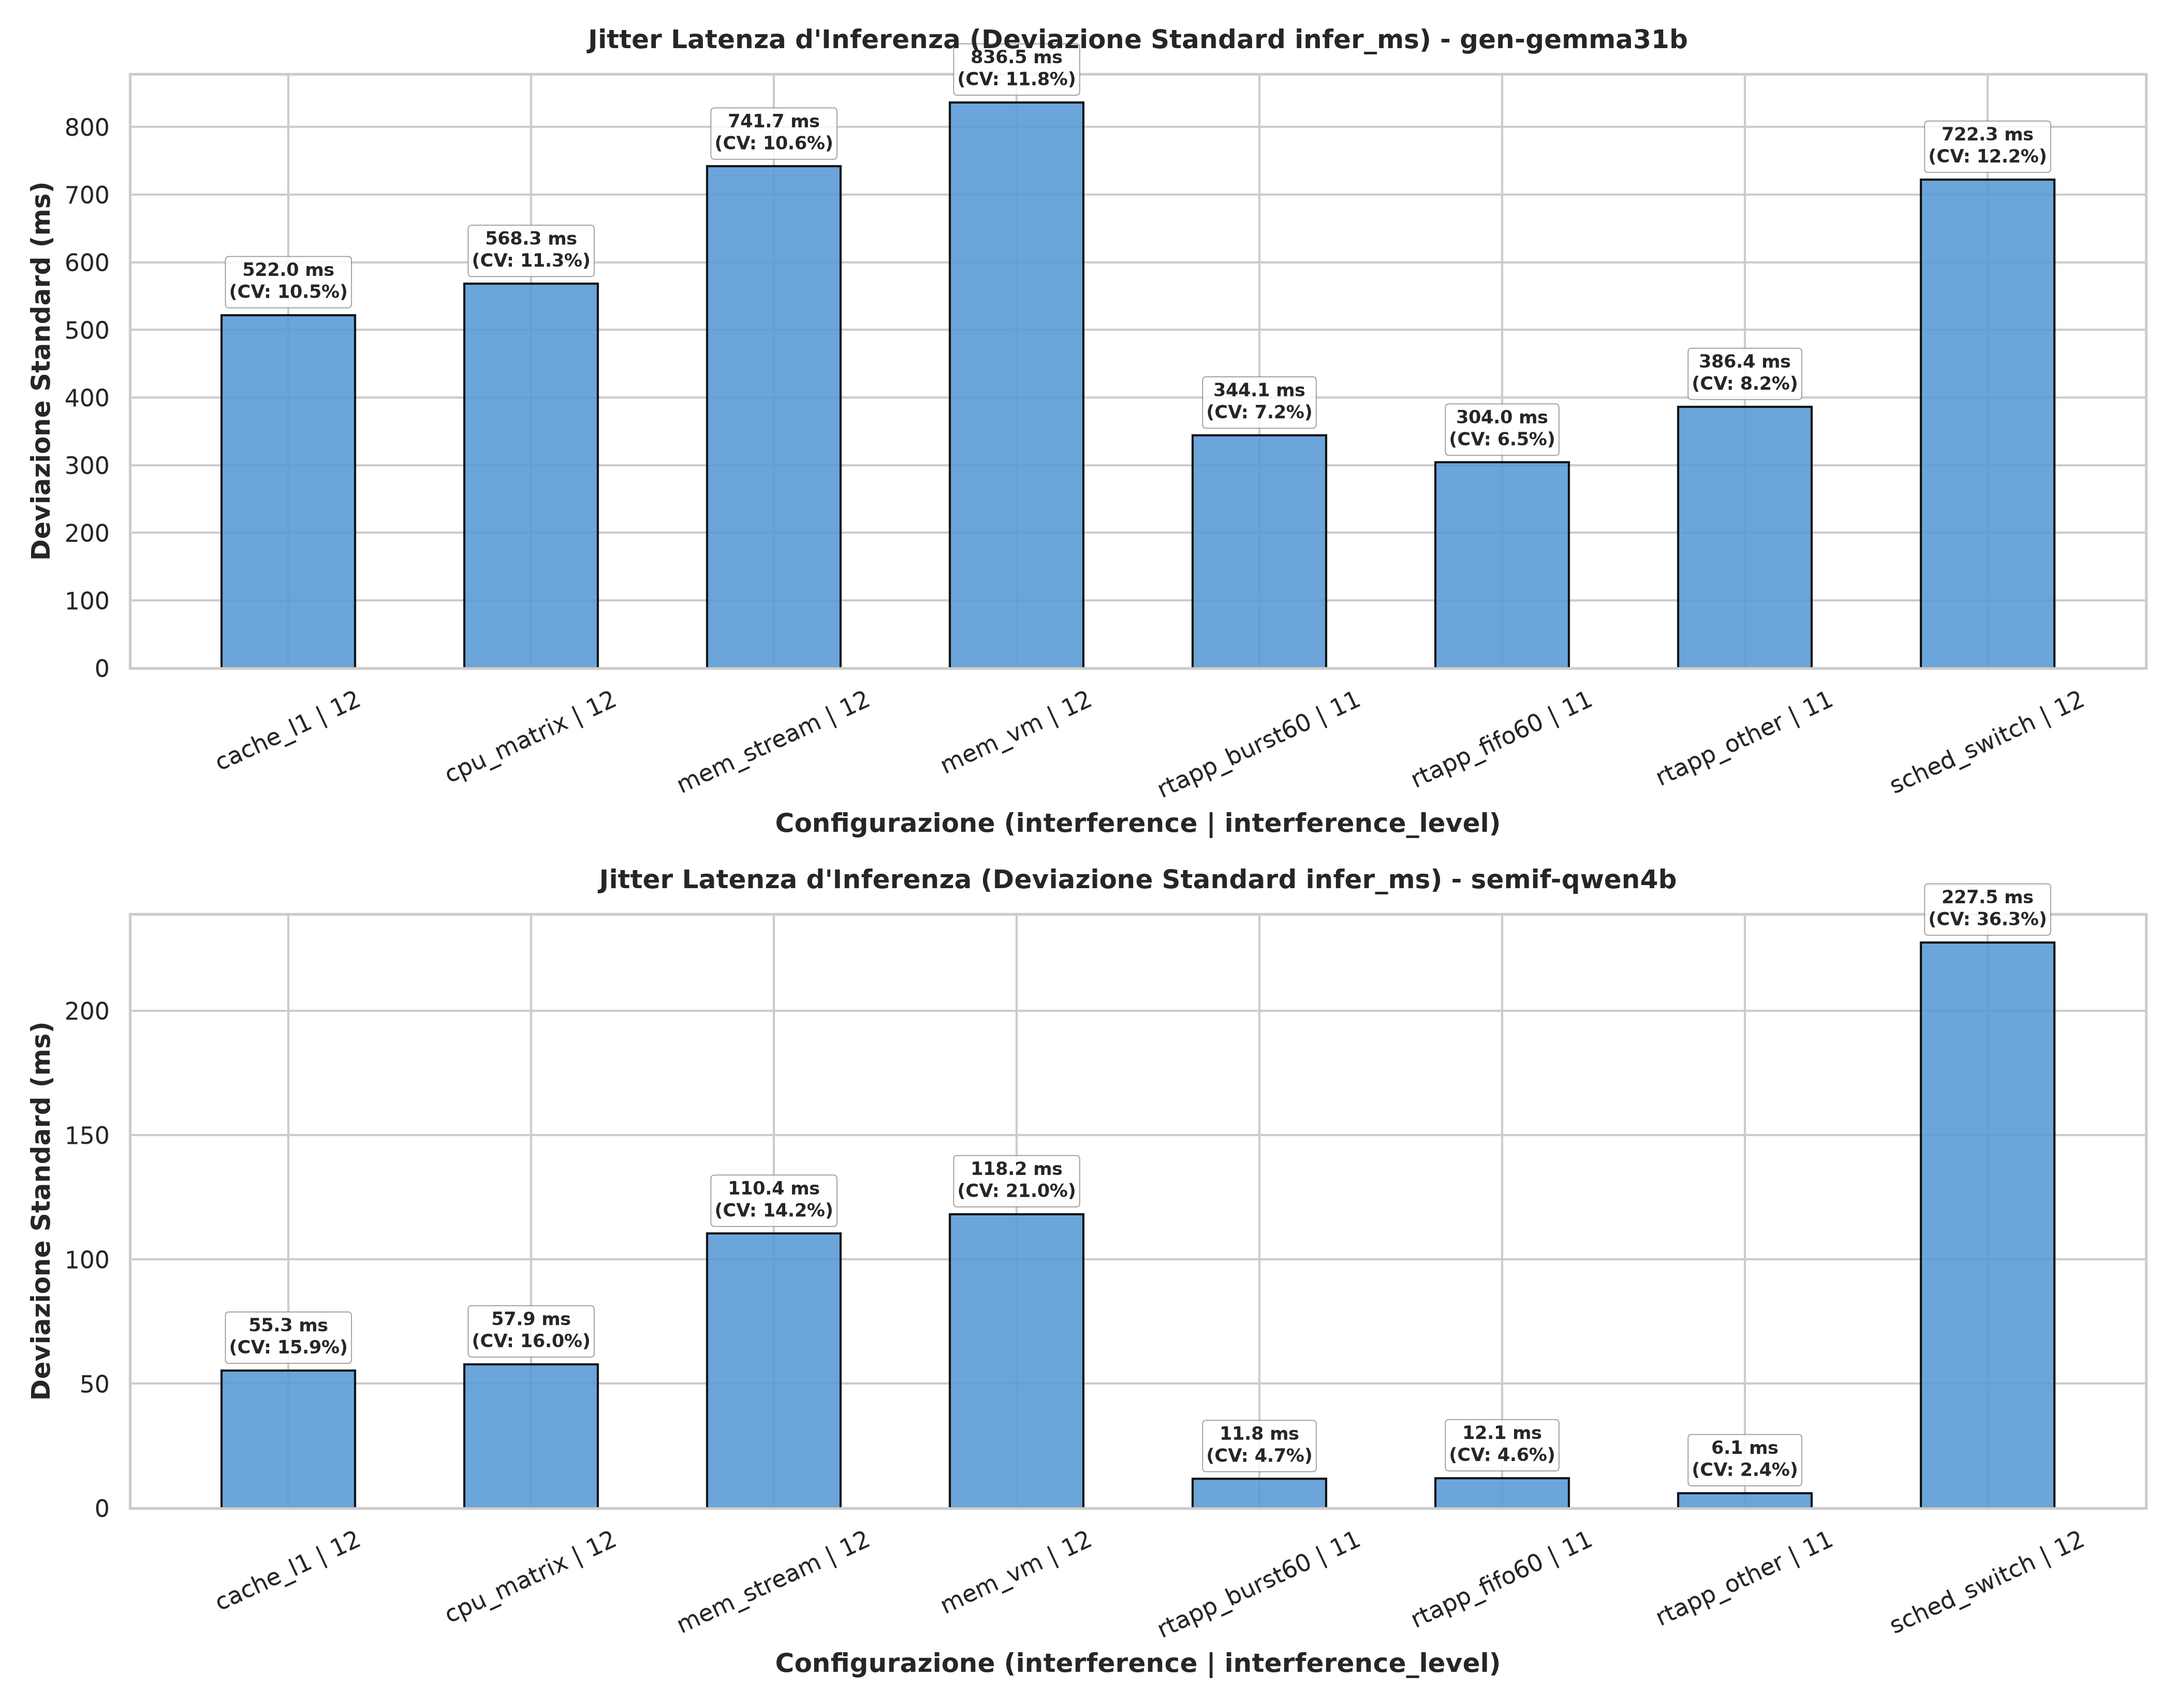
\includegraphics[width=0.97\columnwidth]{plots/markdown/b3_interference/jitter_infer_ms.png}
\caption{B3: jitter e variabilità dell’inferenza sotto interferenza.}\label{fig:b3jitter}
\end{figure}

\FloatBarrier
\subsection{Composizione dell'inferenza e utilizzo delle risorse}
La Fig.~\ref{fig:b3phases} illustra la sensibilità delle fasi di elaborazione ai carichi concorrenti. Il decode di Gemma richiede accessi ripetuti ai parametri e può risentire della contesa della memoria condivisa. Tuttavia, non è possibile attribuire il degrado dei carichi di memoria alla sola saturazione della banda.
Le Figg.~\ref{fig:b3semif} e~\ref{fig:b3gemma}, insieme alla Tabella~\ref{tab:resources}, mostrano un utilizzo elevato della CPU durante \code{mem_stream}. Per SemIf, l'utilizzo medio della GPU è circa 30--31\%, mentre quello della CPU supera il 93\%; per Gemma, la CPU è prossima al 100\% e la GPU presenta valori medi di circa 90--93\%. Queste osservazioni sono compatibili con interferenze nell'orchestrazione CPU dell'inferenza. La distinzione quantitativa tra effetti di scheduling, cache e banda richiederebbe misure dedicate.

\begin{figure}[!htbp]
\centering
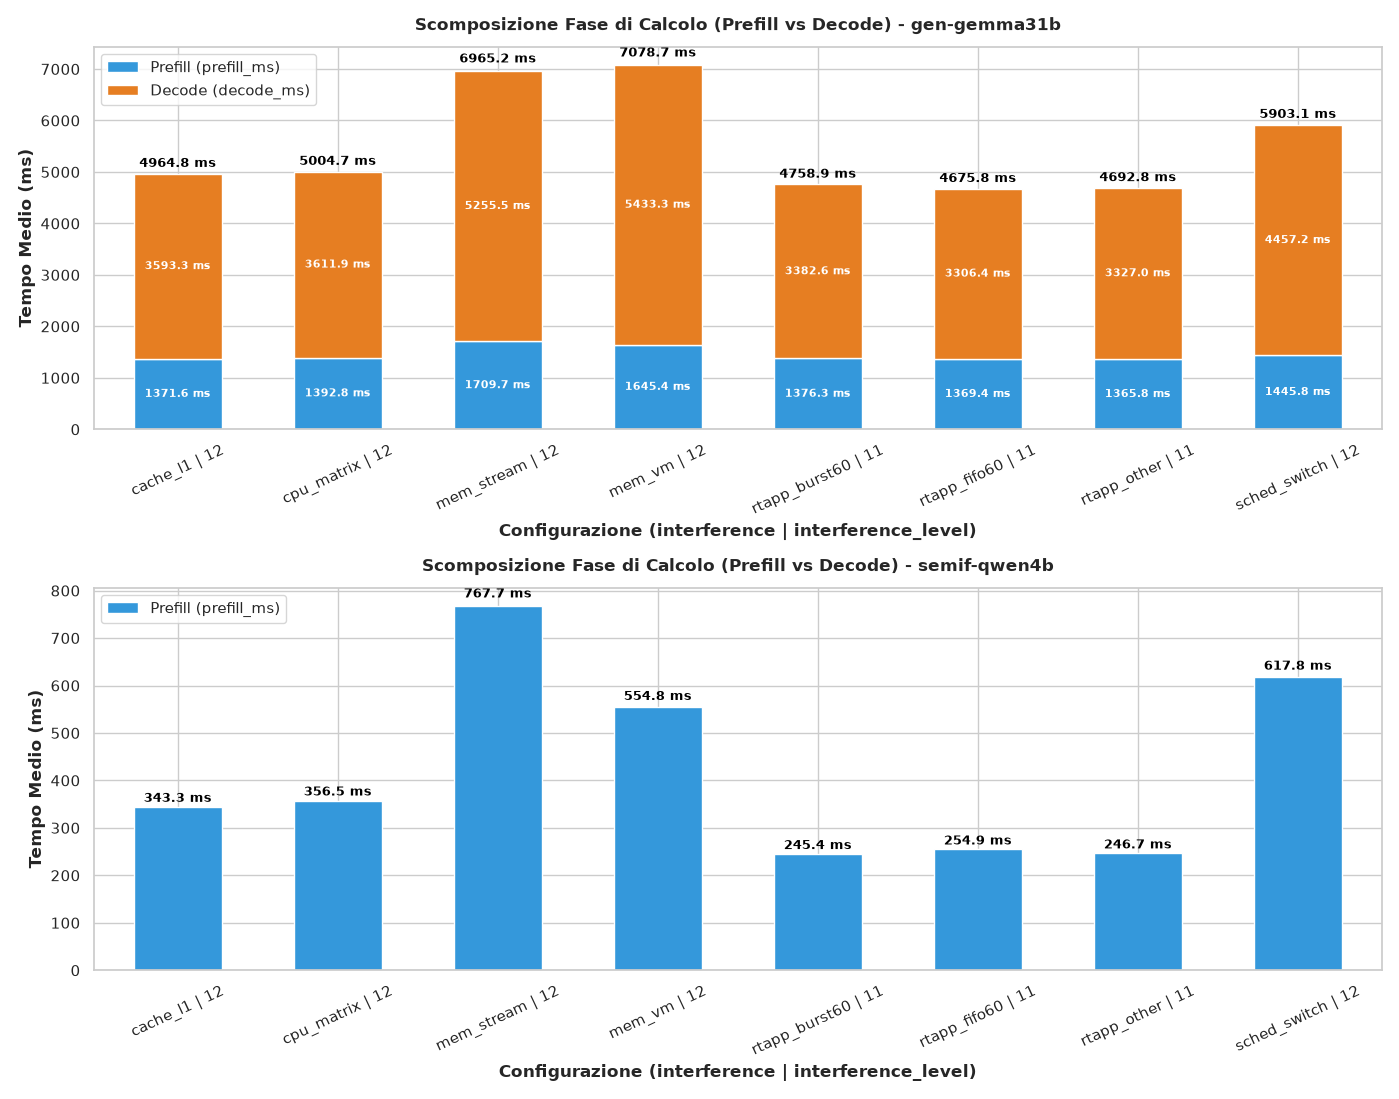
\includegraphics[width=0.97\columnwidth]{plots/markdown/b3_interference/prefill_decode.png}
\caption{B3: ripartizione dei tempi di prefill e decode.}\label{fig:b3phases}
\end{figure}

\begin{figure}[!htbp]
\centering
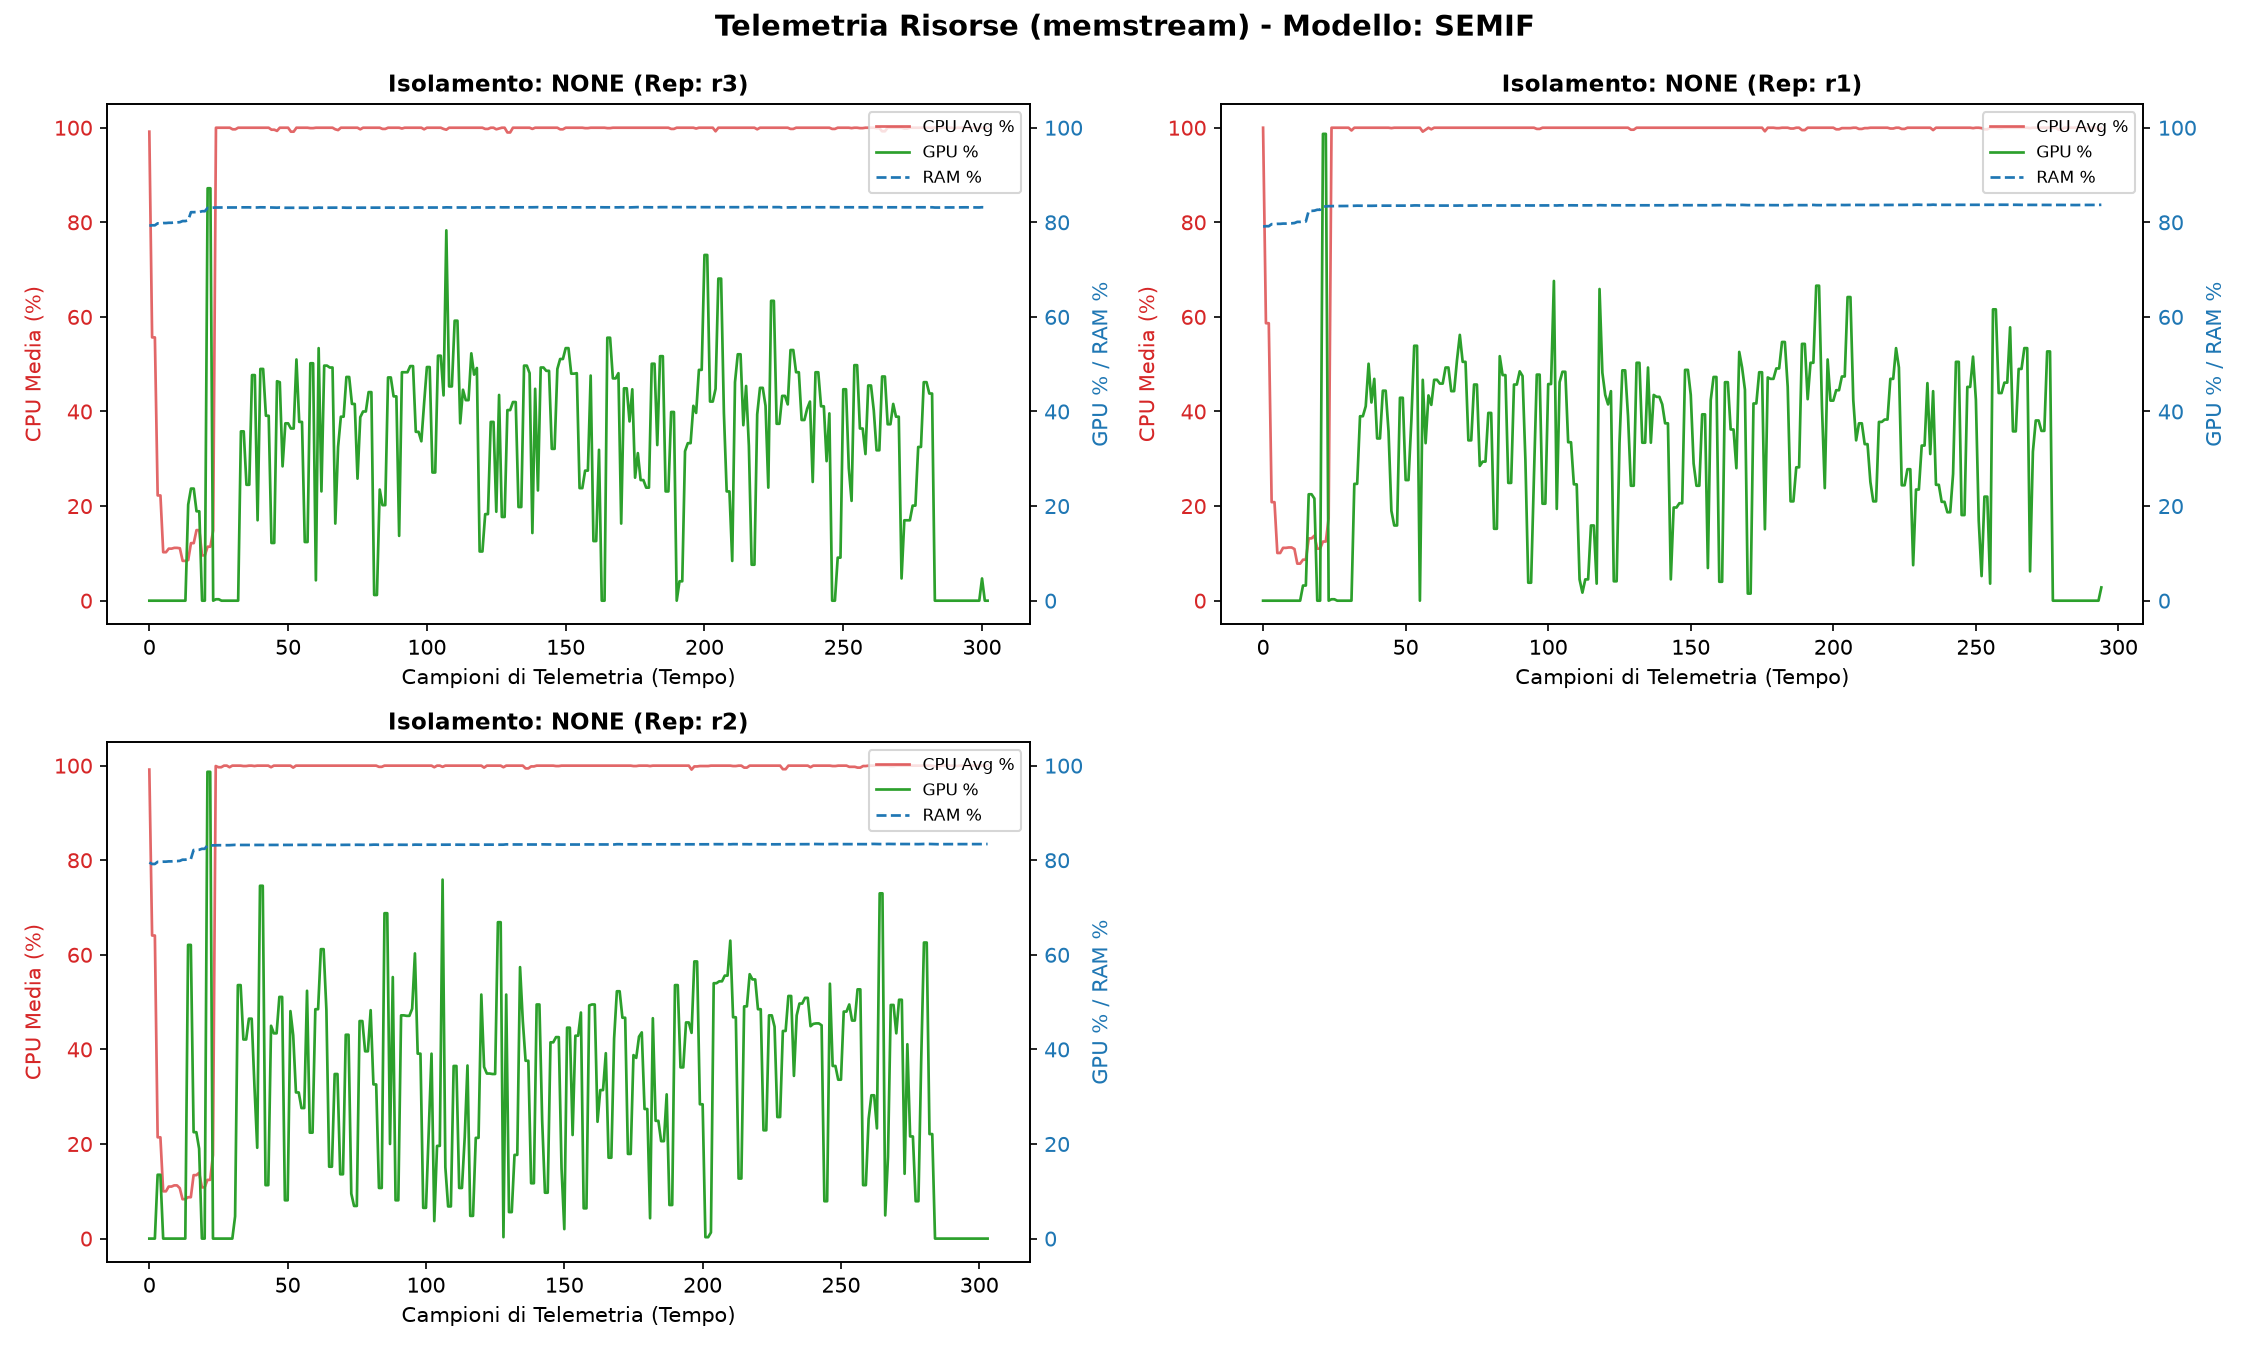
\includegraphics[width=0.97\columnwidth]{plots/markdown/b3_interference/chart_memstream_model_semif.png}
\caption{B3: andamento dell’utilizzo delle risorse per SemIf con carico mem\_stream.}\label{fig:b3semif}
\end{figure}

\begin{figure}[!htbp]
\centering
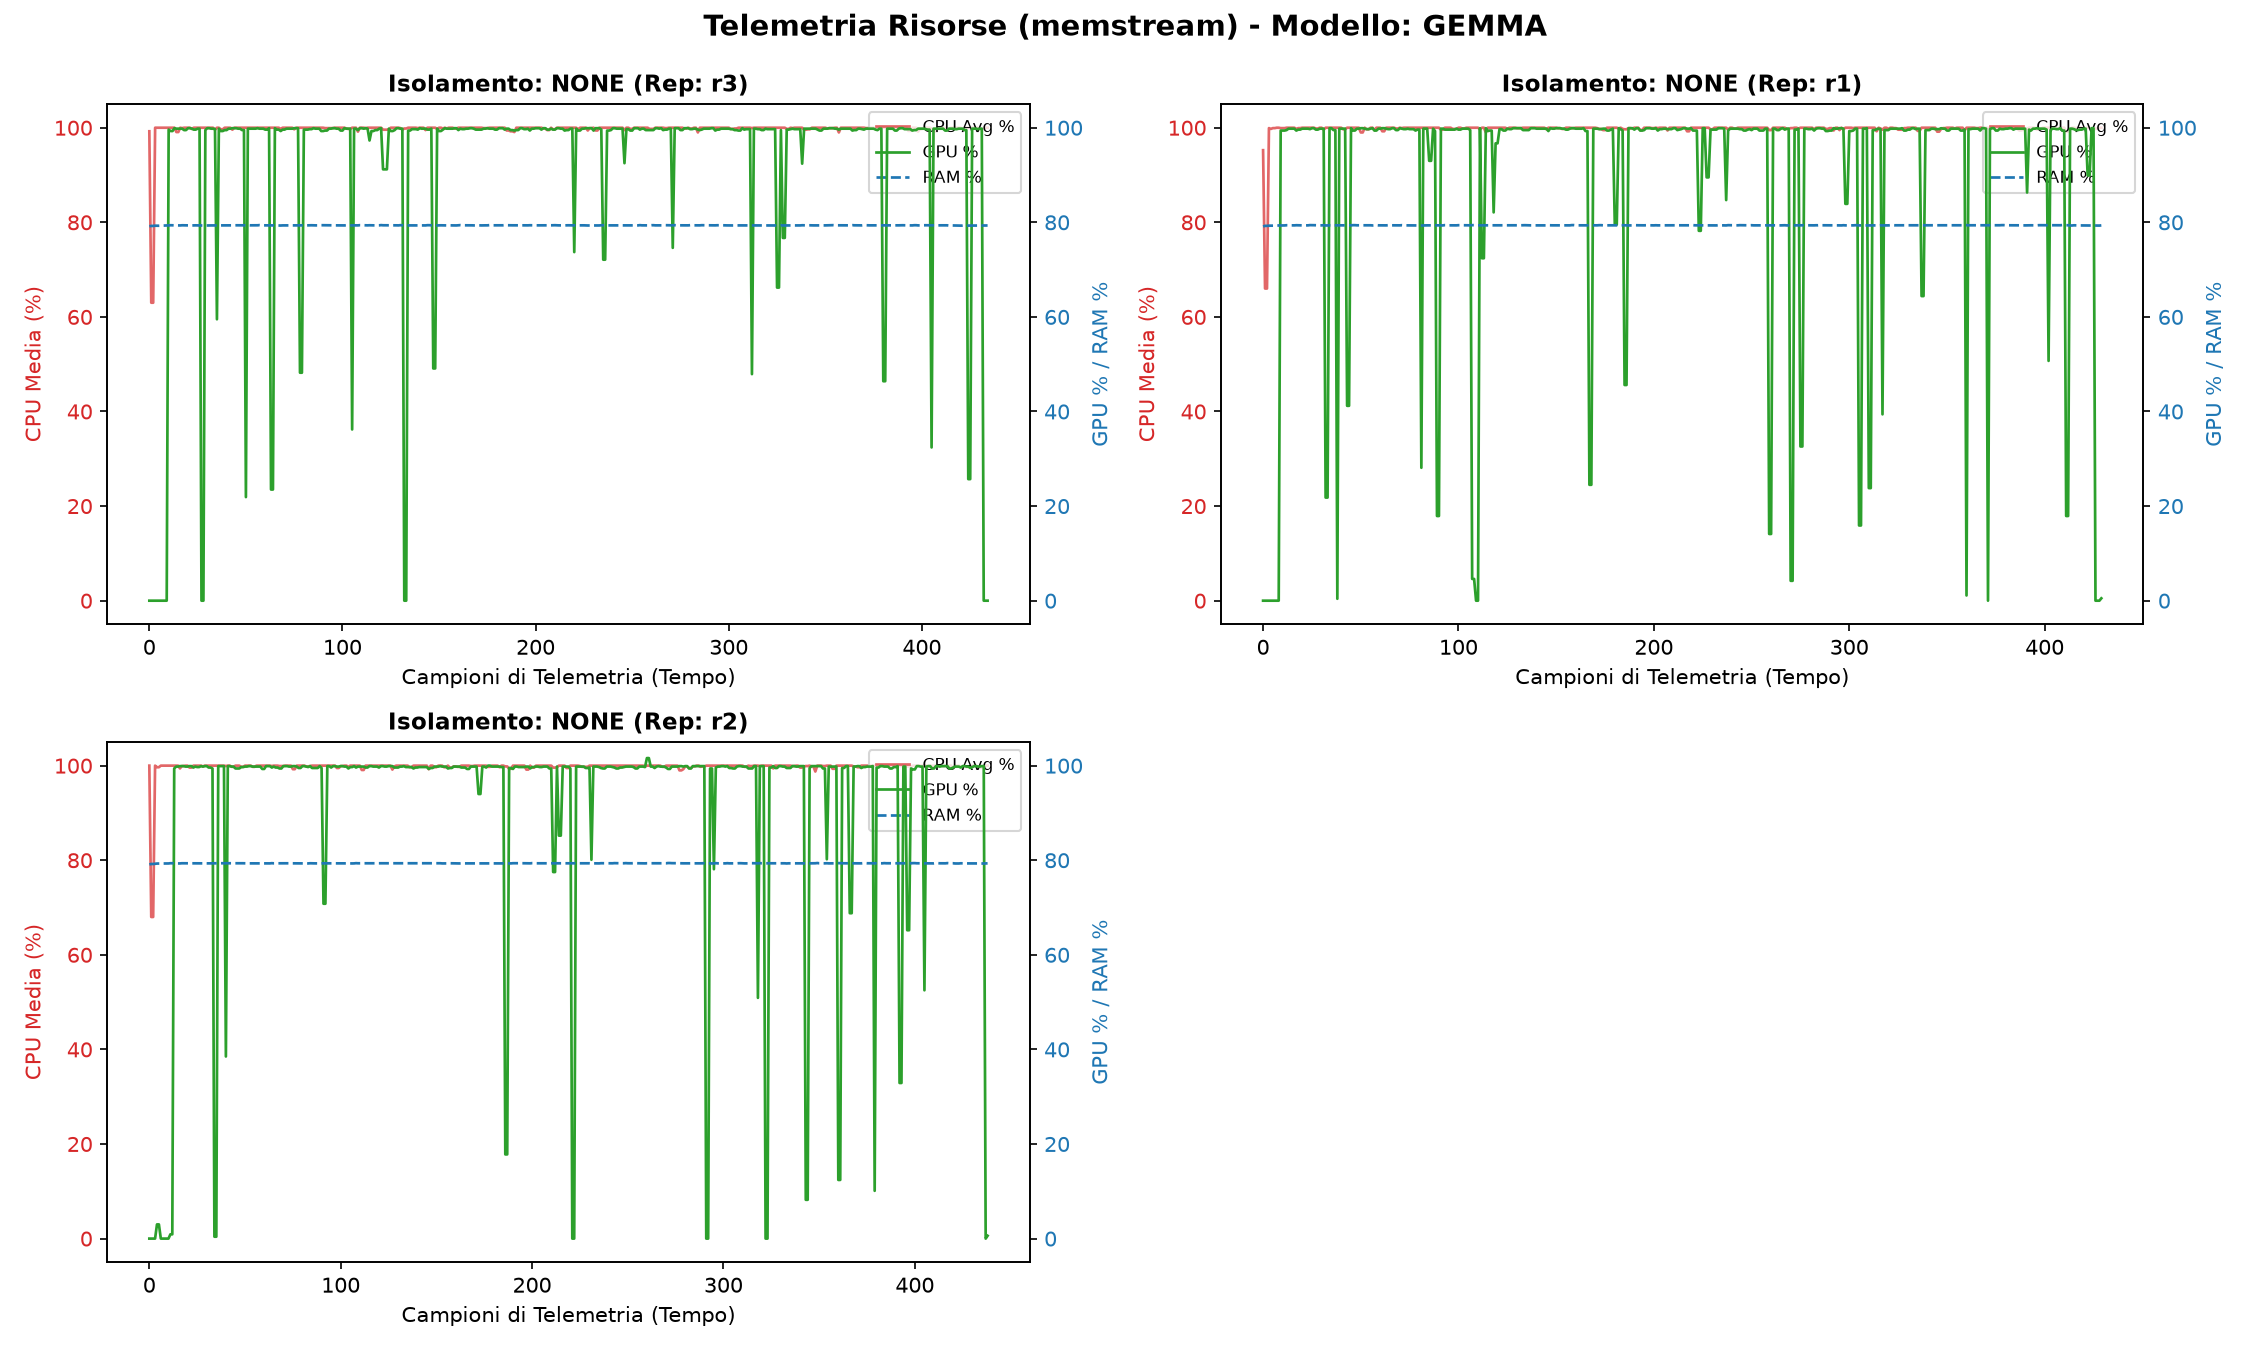
\includegraphics[width=0.97\columnwidth]{plots/markdown/b3_interference/chart_memstream_model_gemma.png}
\caption{B3: andamento dell’utilizzo delle risorse per Gemma con carico mem\_stream.}\label{fig:b3gemma}
\end{figure}

\begin{table*}[!t]
\centering
\caption{Utilizzo delle risorse con mem\_stream senza isolamento; tutte le grandezze di utilizzo sono percentuali.}\label{tab:resources}
\footnotesize
\setlength{\tabcolsep}{4pt}
\begin{tabular}{lllllllll}
\toprule
Sistema & Isolamento & Interferenza & RAM media (\%) & RAM max (\%) & GPU media (\%) & GPU max (\%) & CPU media (\%) & CPU max (\%) \\
\midrule
Semif & none & mem\_stream & 82.97 & 83.23 & 31.42 & 87.2 & 93.57 & 100 \\
Semif & none & mem\_stream & 83.38 & 83.73 & 31.07 & 98.7 & 93.43 & 100 \\
Semif & none & mem\_stream & 83.13 & 83.46 & 30.51 & 98.7 & 93.66 & 100 \\
Gemma & none & mem\_stream & 79.35 & 79.41 & 93.11 & 99.9 & 99.75 & 100 \\
Gemma & none & mem\_stream & 79.36 & 79.42 & 89.98 & 99.9 & 99.74 & 100 \\
Gemma & none & mem\_stream & 79.35 & 79.41 & 91.71 & 100 & 99.76 & 100 \\
\bottomrule
\end{tabular}
\end{table*}

\FloatBarrier
\section{B4. Isolamento}\label{sec:b4}

\FloatBarrier
\subsection{Configurazione e piano sperimentale}
B4 valuta tecniche di isolamento rispetto ai carichi maggiormente penalizzanti identificati in B3. La CPU della piattaforma comprende 12 core dello stesso tipo; non viene quindi adottata una distinzione tra core ad alte prestazioni e core ad alta efficienza.
La configurazione adottata riserva i core 0--7 ai modelli e all'infrastruttura ROS, mediante \code{isolcpus}, \code{nohz_full} e \code{rcu_nocbs}, e indirizza le interruzioni ai core 8--11 con \code{irqaffinity=8-11}. Tali parametri mirano a ridurre le interferenze del kernel sui core riservati, ma non dimostrano da soli l'assenza di ogni interruzione o attività di sistema.
Sono confrontate tre modalità: \code{pin}, ossia affinità dei processi ai core isolati; \code{prio}, ossia incremento della priorità; e \code{pin_prio}, ossia combinazione delle due tecniche. La Tabella~\ref{tab:b4} riporta il piano, con tre ripetizioni per configurazione.

\begin{table}[!htbp]
\centering
\caption{Piano sperimentale B4: interferenze e tecniche di isolamento.}\label{tab:b4}
\scriptsize
\setlength{\tabcolsep}{2pt}
\begin{tabular}{lllllll}
\toprule
Sistema & Carico & Liv. & Isolamento & Rep. & $t$ (s) & $f$ (Hz) \\
\midrule
semif & mem\_stream & 12 & pin & 3 & 180 & 2 \\
semif & mem\_stream & 12 & prio & 3 & 180 & 2 \\
semif & mem\_stream & 12 & pin\_prio & 3 & 180 & 2 \\
semif & mem\_vm & 12 & pin & 3 & 180 & 2 \\
semif & mem\_vm & 12 & prio & 3 & 180 & 2 \\
semif & mem\_vm & 12 & pin\_prio & 3 & 180 & 2 \\
semif & sched\_switch & 12 & pin & 3 & 180 & 2 \\
semif & sched\_switch & 12 & prio & 3 & 180 & 2 \\
semif & sched\_switch & 12 & pin\_prio & 3 & 180 & 2 \\
gemma & mem\_stream & 12 & pin & 3 & 300 & 2 \\
gemma & mem\_stream & 12 & prio & 3 & 300 & 2 \\
gemma & mem\_stream & 12 & pin\_prio & 3 & 300 & 2 \\
gemma & sched\_switch & 12 & pin & 3 & 300 & 2 \\
gemma & sched\_switch & 12 & prio & 3 & 300 & 2 \\
gemma & sched\_switch & 12 & pin\_prio & 3 & 300 & 2 \\
gemma & mem\_vm & 12 & pin & 3 & 300 & 2 \\
gemma & mem\_vm & 12 & prio & 3 & 300 & 2 \\
gemma & mem\_vm & 12 & pin\_prio & 3 & 300 & 2 \\
\bottomrule
\end{tabular}
\end{table}

\FloatBarrier
\subsection{Latenza end-to-end e inferenza}
Le Figg.~\ref{fig:b4e2e} e~\ref{fig:b4inf} mostrano un recupero delle prestazioni verso i valori osservati a riposo. Il pinning sui core isolati risulta la tecnica più efficace tra quelle considerate, mentre il solo incremento della priorità produce benefici più limitati.

\begin{figure}[!htbp]
\centering
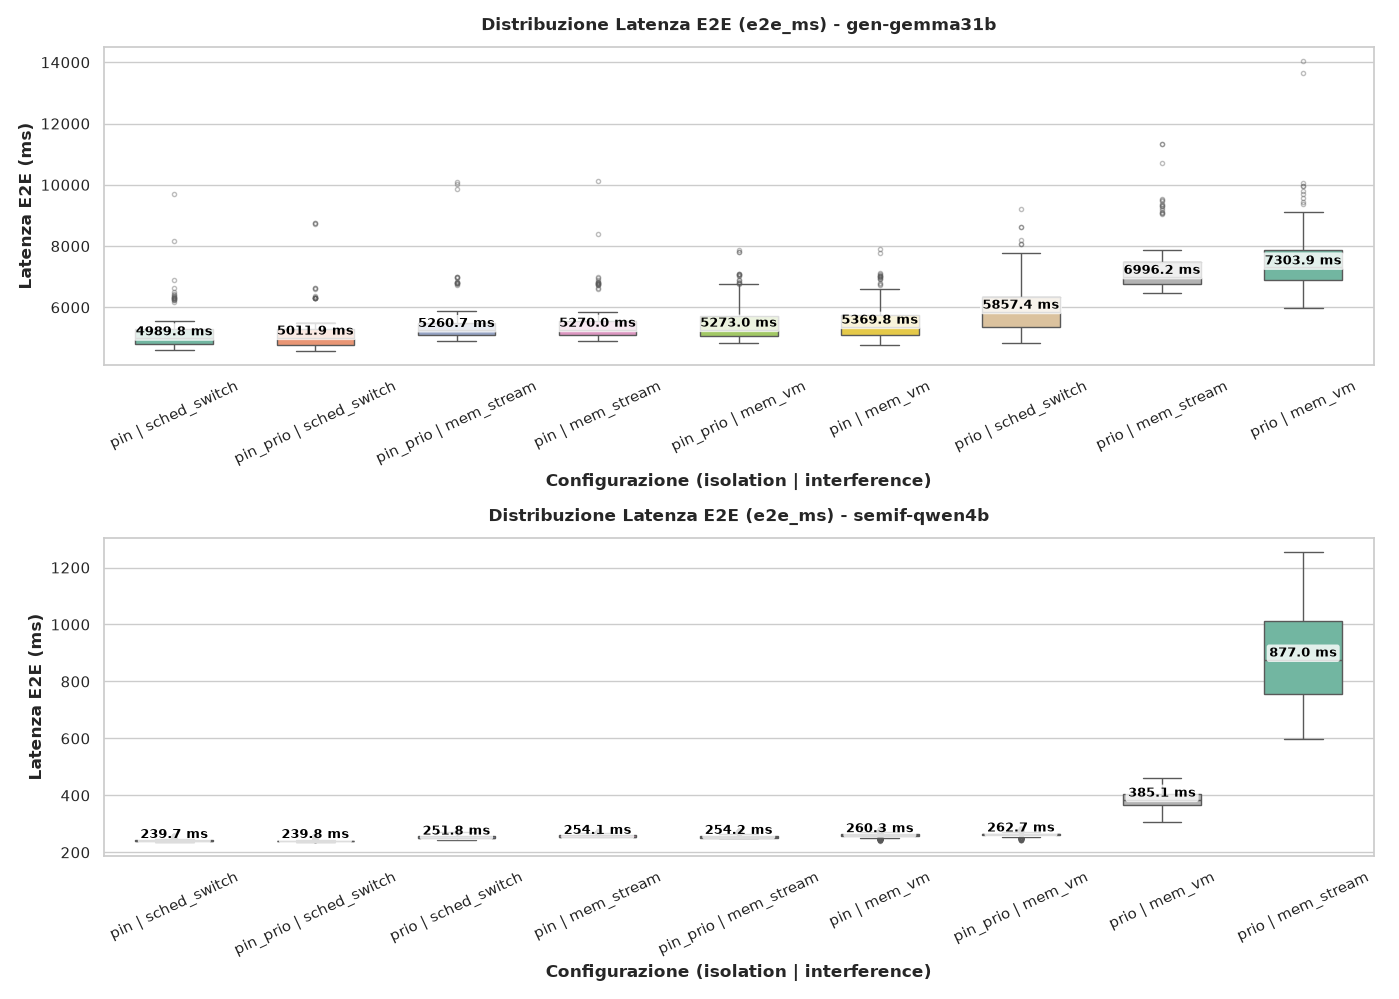
\includegraphics[width=0.97\columnwidth]{plots/markdown/b4_isolation/Box_plots_e2e.png}
\caption{B4: effetto delle tecniche di isolamento sulla latenza end-to-end.}\label{fig:b4e2e}
\end{figure}

\begin{figure}[!htbp]
\centering
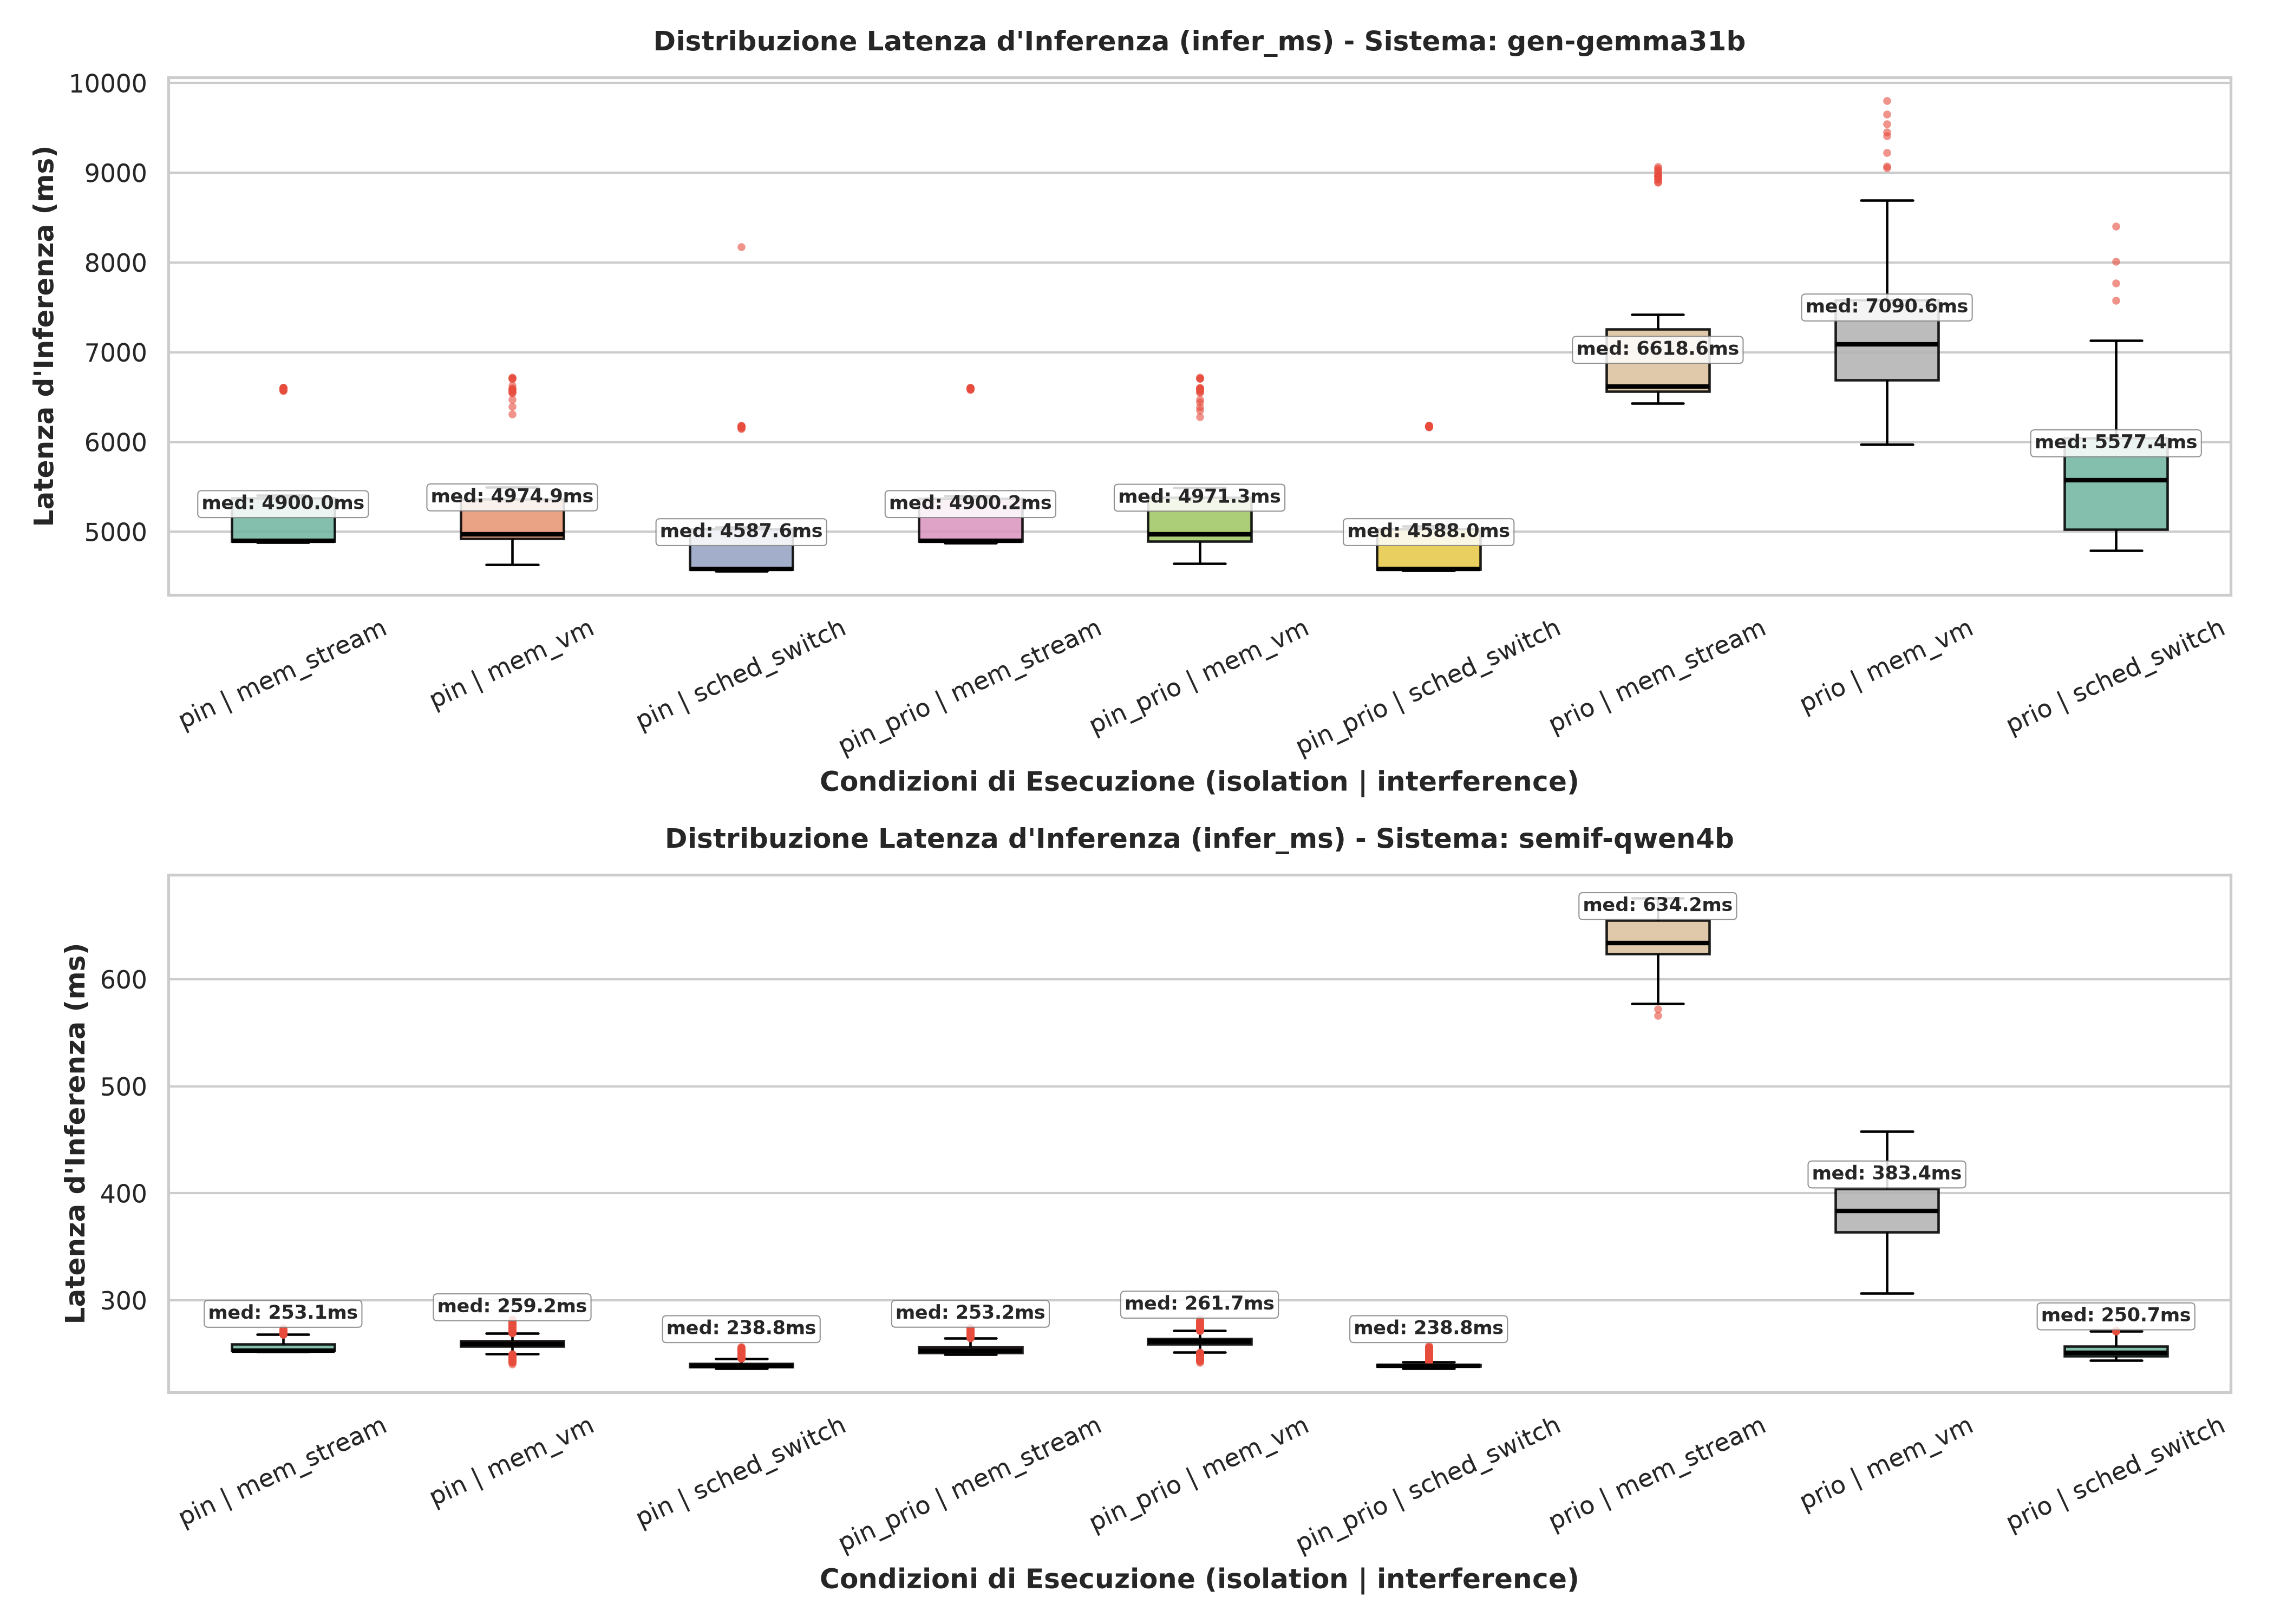
\includegraphics[width=0.97\columnwidth]{plots/markdown/b4_isolation/boxplot_infer_ms.png}
\caption{B4: effetto dell’isolamento sulla latenza di inferenza.}\label{fig:b4inf}
\end{figure}

\FloatBarrier
\subsection{Latenze di coda e stabilità}
Le latenze di coda e il jitter sono riportati nelle Figg.~\ref{fig:b4tail} e~\ref{fig:b4jitter}. Gemma conserva picchi che possono raggiungere circa 8 s, pur presentando una variabilità dell'inferenza più contenuta rispetto al caso senza isolamento. Per SemIf, il pinning limita le variazioni del jitter a pochi millisecondi.

\begin{figure}[!htbp]
\centering
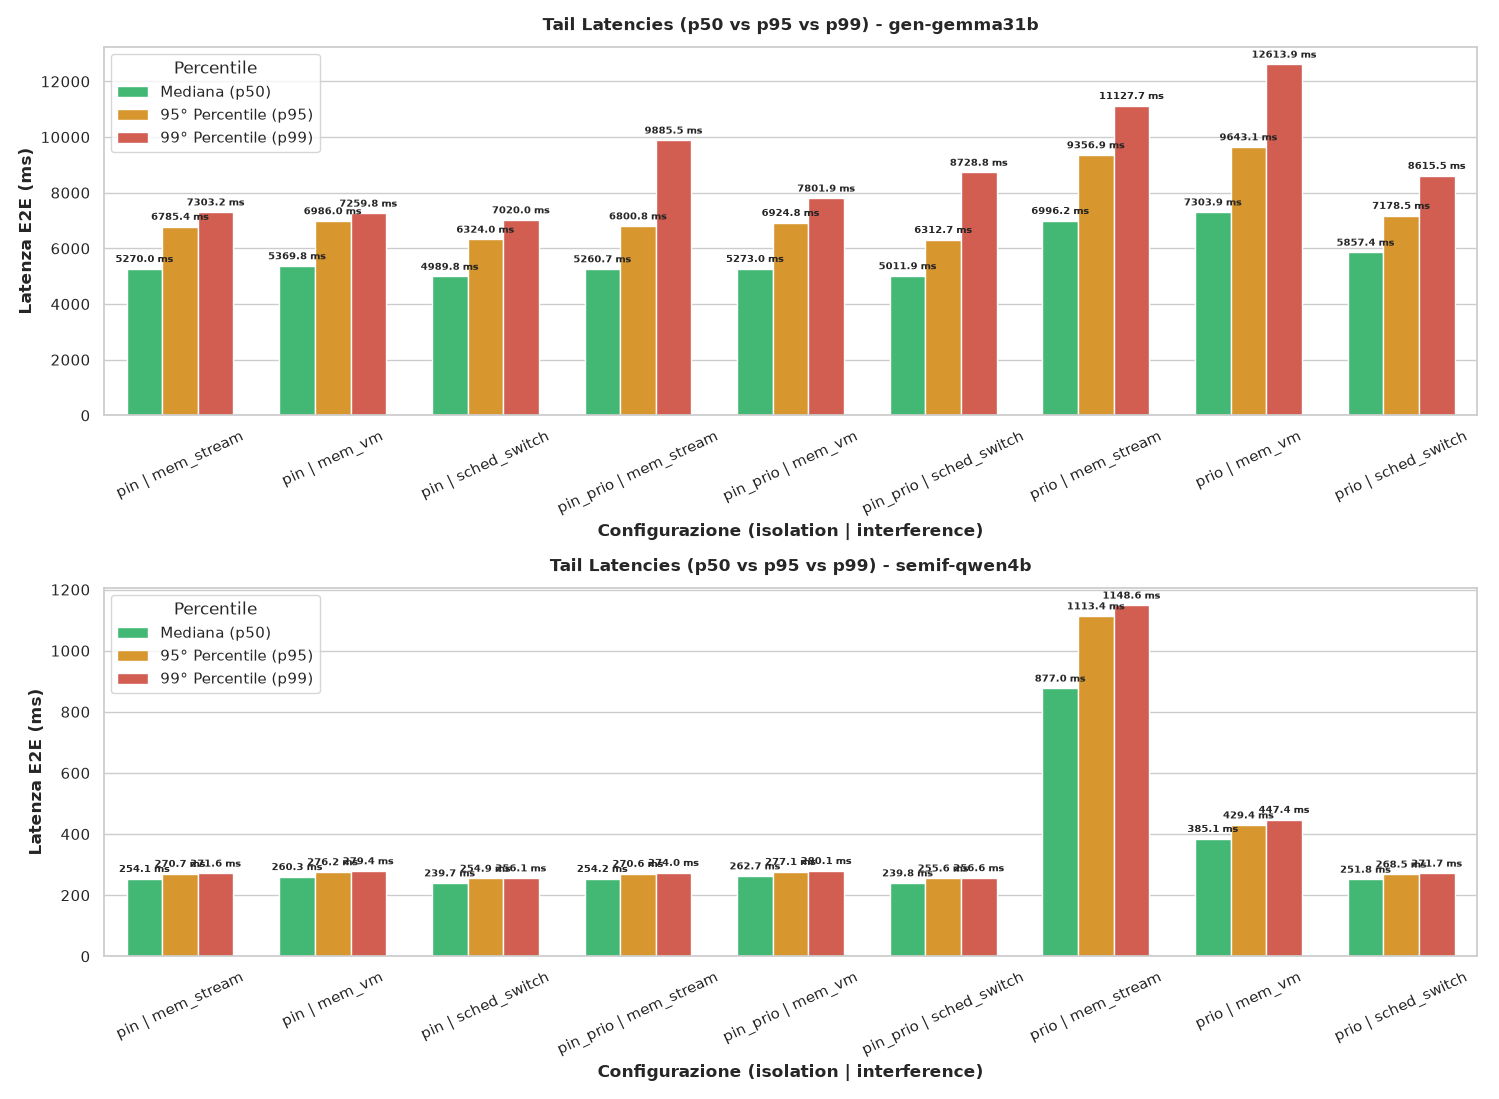
\includegraphics[width=0.97\columnwidth]{plots/markdown/b4_isolation/tail_latencies.png}
\caption{B4: latenze di coda con isolamento.}\label{fig:b4tail}
\end{figure}

\begin{figure}[!htbp]
\centering
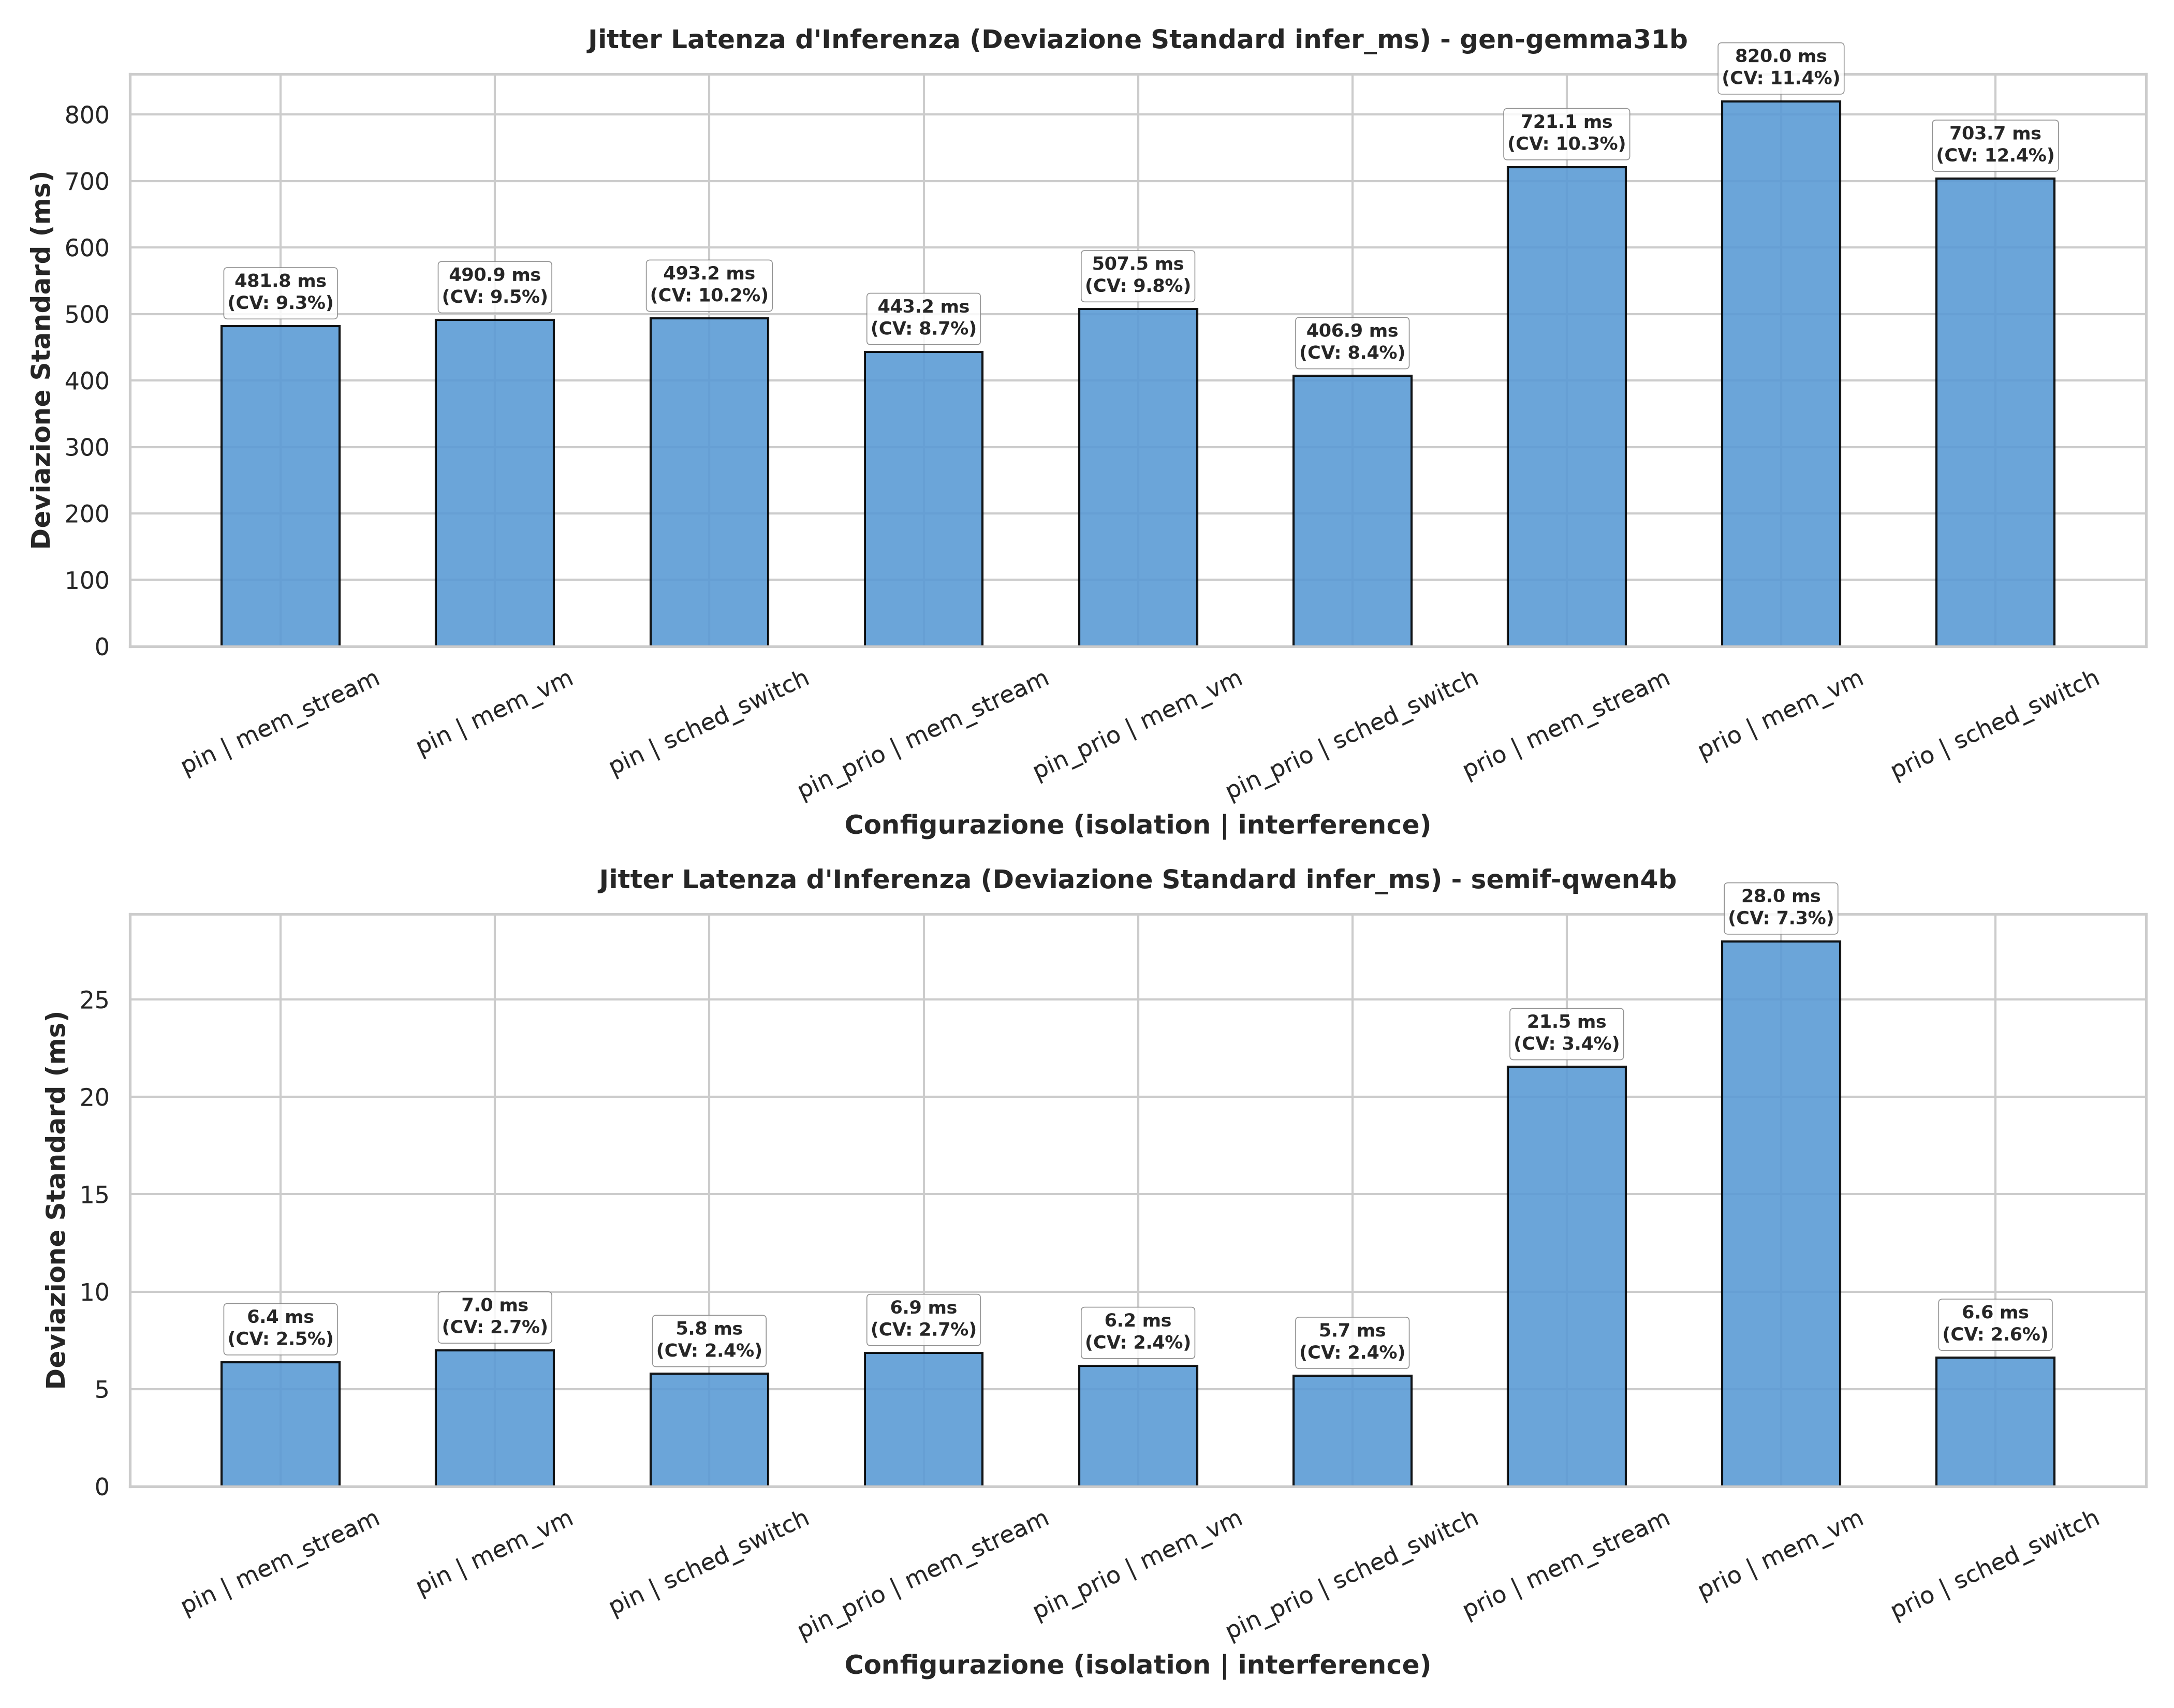
\includegraphics[width=0.97\columnwidth]{plots/markdown/b4_isolation/jitter_infer_ms.png}
\caption{B4: jitter e variabilità dell’inferenza con isolamento.}\label{fig:b4jitter}
\end{figure}

\FloatBarrier
\subsection{Interpretazione dei risultati}
Il recupero osservato con carichi di memoria suggerisce un ruolo rilevante della contesa sui core CPU, oltre a quello della memoria condivisa. La separazione dei processi può ridurre le preemption e la perturbazione delle cache private. La banda nominale della memoria LPDDR5 è pari a 204,8 GB/s, mentre il traffico generato dai quattro worker effettivi sui core residui è stimato in circa 30 GB/s. Questi valori contestualizzano il risultato, ma non costituiscono una misura completa della contesa CPU/GPU.
L'isolamento modifica anche le risorse CPU disponibili agli stressori: a parità di livello configurato, il carico effettivo può differire da B3. Il miglioramento non va quindi interpretato come effetto esclusivo dell'eliminazione dei cambi di contesto.

\FloatBarrier
\section{B5. Isolamento e co-locazione}\label{sec:b5}

\FloatBarrier
\subsection{Piano sperimentale}
B5 verifica se le tecniche di isolamento della CPU migliorano il comportamento dei modelli in co-locazione sulla GPU. Sono considerate l'applicazione delle tecniche a entrambi i modelli e l'applicazione a un solo modello, identificata dai suffissi \code{@semif} e \code{@gemma}. Il piano comprende anche una configurazione senza isolamento e prevede tre ripetizioni da 300 s per ogni caso (Tabella~\ref{tab:b5}). Non sono introdotti stressori aggiuntivi.

\begin{table}[!htbp]
\centering
\caption{Piano sperimentale B5: isolamento congiunto e selettivo in co-locazione.}\label{tab:b5}
\scriptsize
\setlength{\tabcolsep}{2pt}
\begin{tabular}{lllllll}
\toprule
Sistema & Carico & Liv. & Isolamento & Rep. & $t$ (s) & $f$ (Hz) \\
\midrule
semif,gemma & none & 0 & pin & 3 & 300 & 2 \\
semif,gemma & none & 0 & prio & 3 & 300 & 2 \\
semif,gemma & none & 0 & pin\_prio & 3 & 300 & 2 \\
semif,gemma & none & 0 & pin@semif & 3 & 300 & 2 \\
semif,gemma & none & 0 & prio@semif & 3 & 300 & 2 \\
semif,gemma & none & 0 & pin\_prio@semif & 3 & 300 & 2 \\
semif,gemma & none & 0 & pin@gemma & 3 & 300 & 2 \\
semif,gemma & none & 0 & prio@gemma & 3 & 300 & 2 \\
semif,gemma & none & 0 & pin\_prio@gemma & 3 & 300 & 2 \\
semif,gemma & none & 0 & none & 3 & 300 & 2 \\
\bottomrule
\end{tabular}
\end{table}

\FloatBarrier
\subsection{Latenze e stabilità}
Le distribuzioni delle Figg.~\ref{fig:b5inf} e~\ref{fig:b5e2e} non mostrano un miglioramento sostanziale delle latenze tra le tecniche considerate e il caso privo di isolamento.


\begin{figure}[!htbp]
\centering
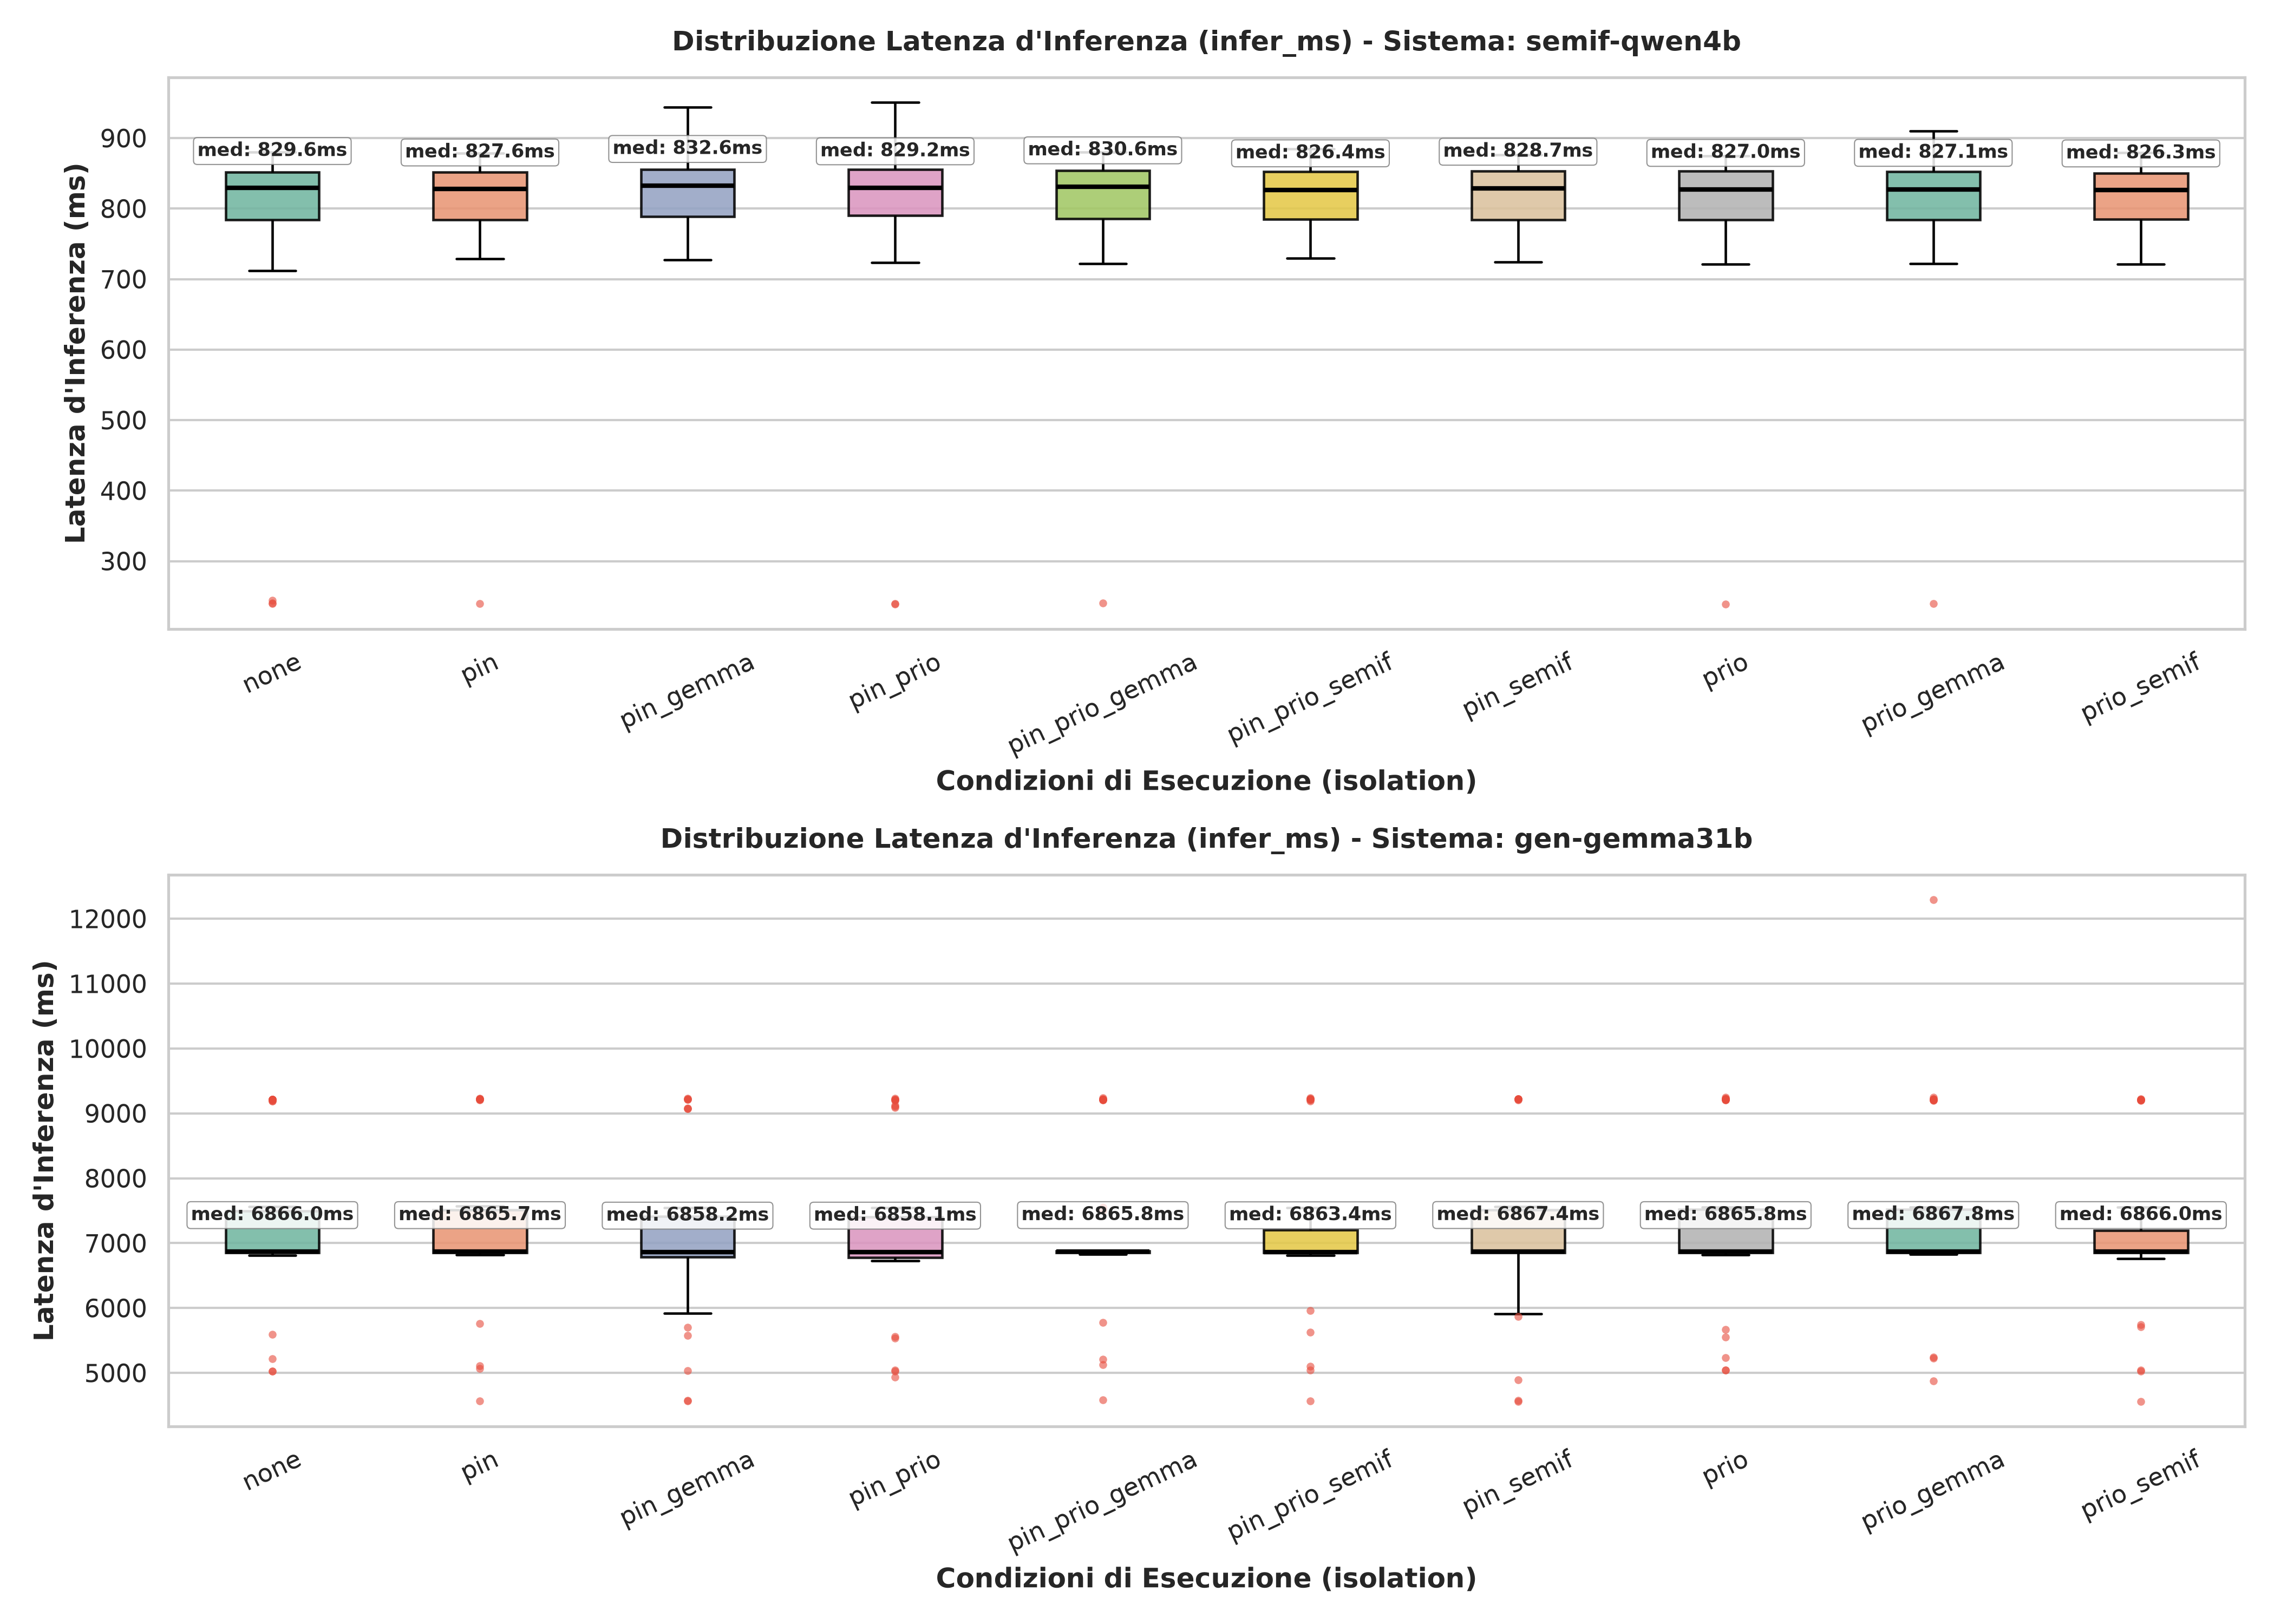
\includegraphics[width=0.97\columnwidth]{plots/markdown/b5_isolation_co_location/boxplot_infer_ms.png}
\caption{B5: latenza di inferenza con isolamento in co-locazione.}\label{fig:b5inf}
\end{figure}

\begin{figure}[!htbp]
\centering
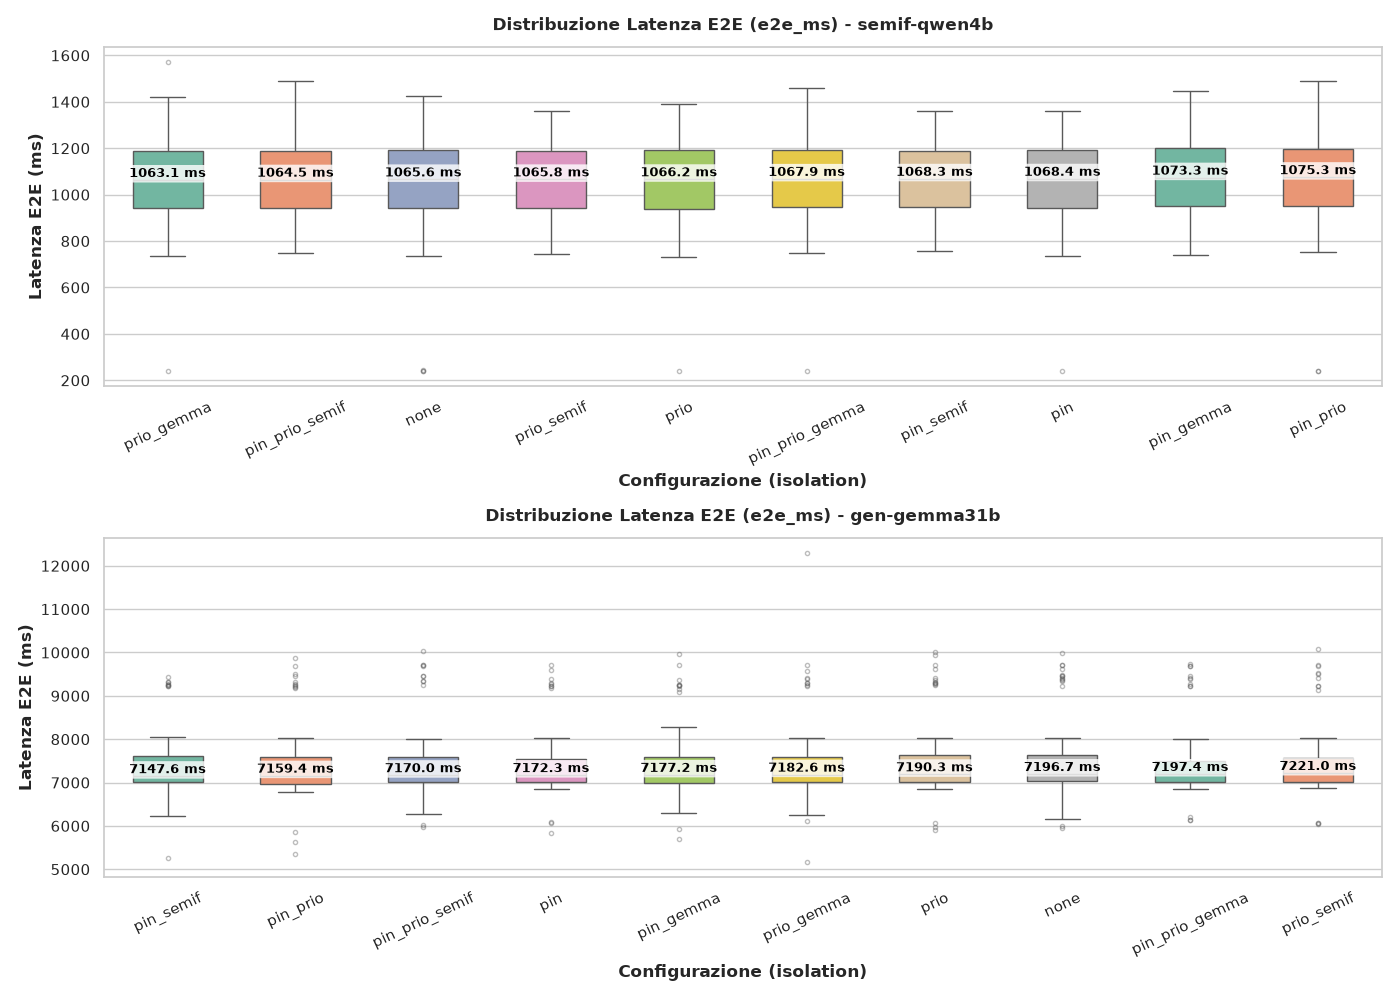
\includegraphics[width=0.97\columnwidth]{plots/markdown/b5_isolation_co_location/Boxplots_e2e.png}
\caption{B5: latenza end-to-end con isolamento in co-locazione.}\label{fig:b5e2e}
\end{figure}

\FloatBarrier
\subsection{Latenze di coda e stabilità}
Le latenze di coda e il jitter (Figg.~\ref{fig:b5tail} e~\ref{fig:b5jitter}) non evidenziano un recupero rilevante della stabilità.

\begin{figure}[!htbp]
\centering
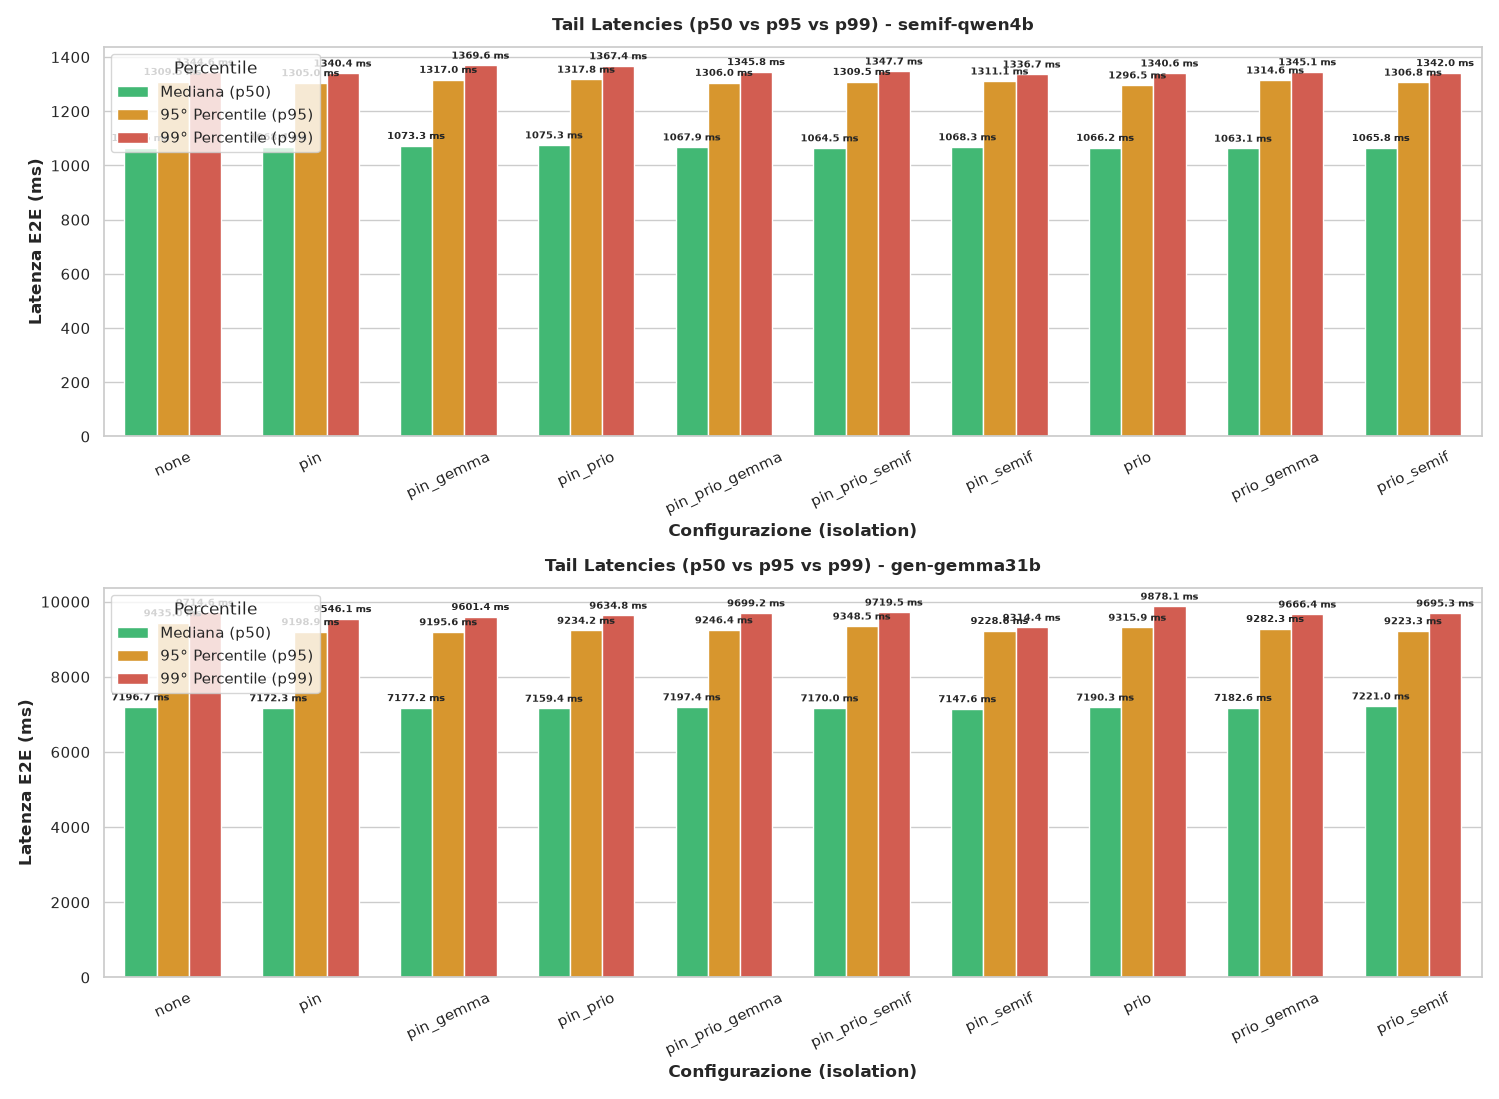
\includegraphics[width=0.97\columnwidth]{plots/markdown/b5_isolation_co_location/Tail_latencies.png}
\caption{B5: latenze di coda con isolamento in co-locazione.}\label{fig:b5tail}
\end{figure}

\begin{figure}[!htbp]
\centering
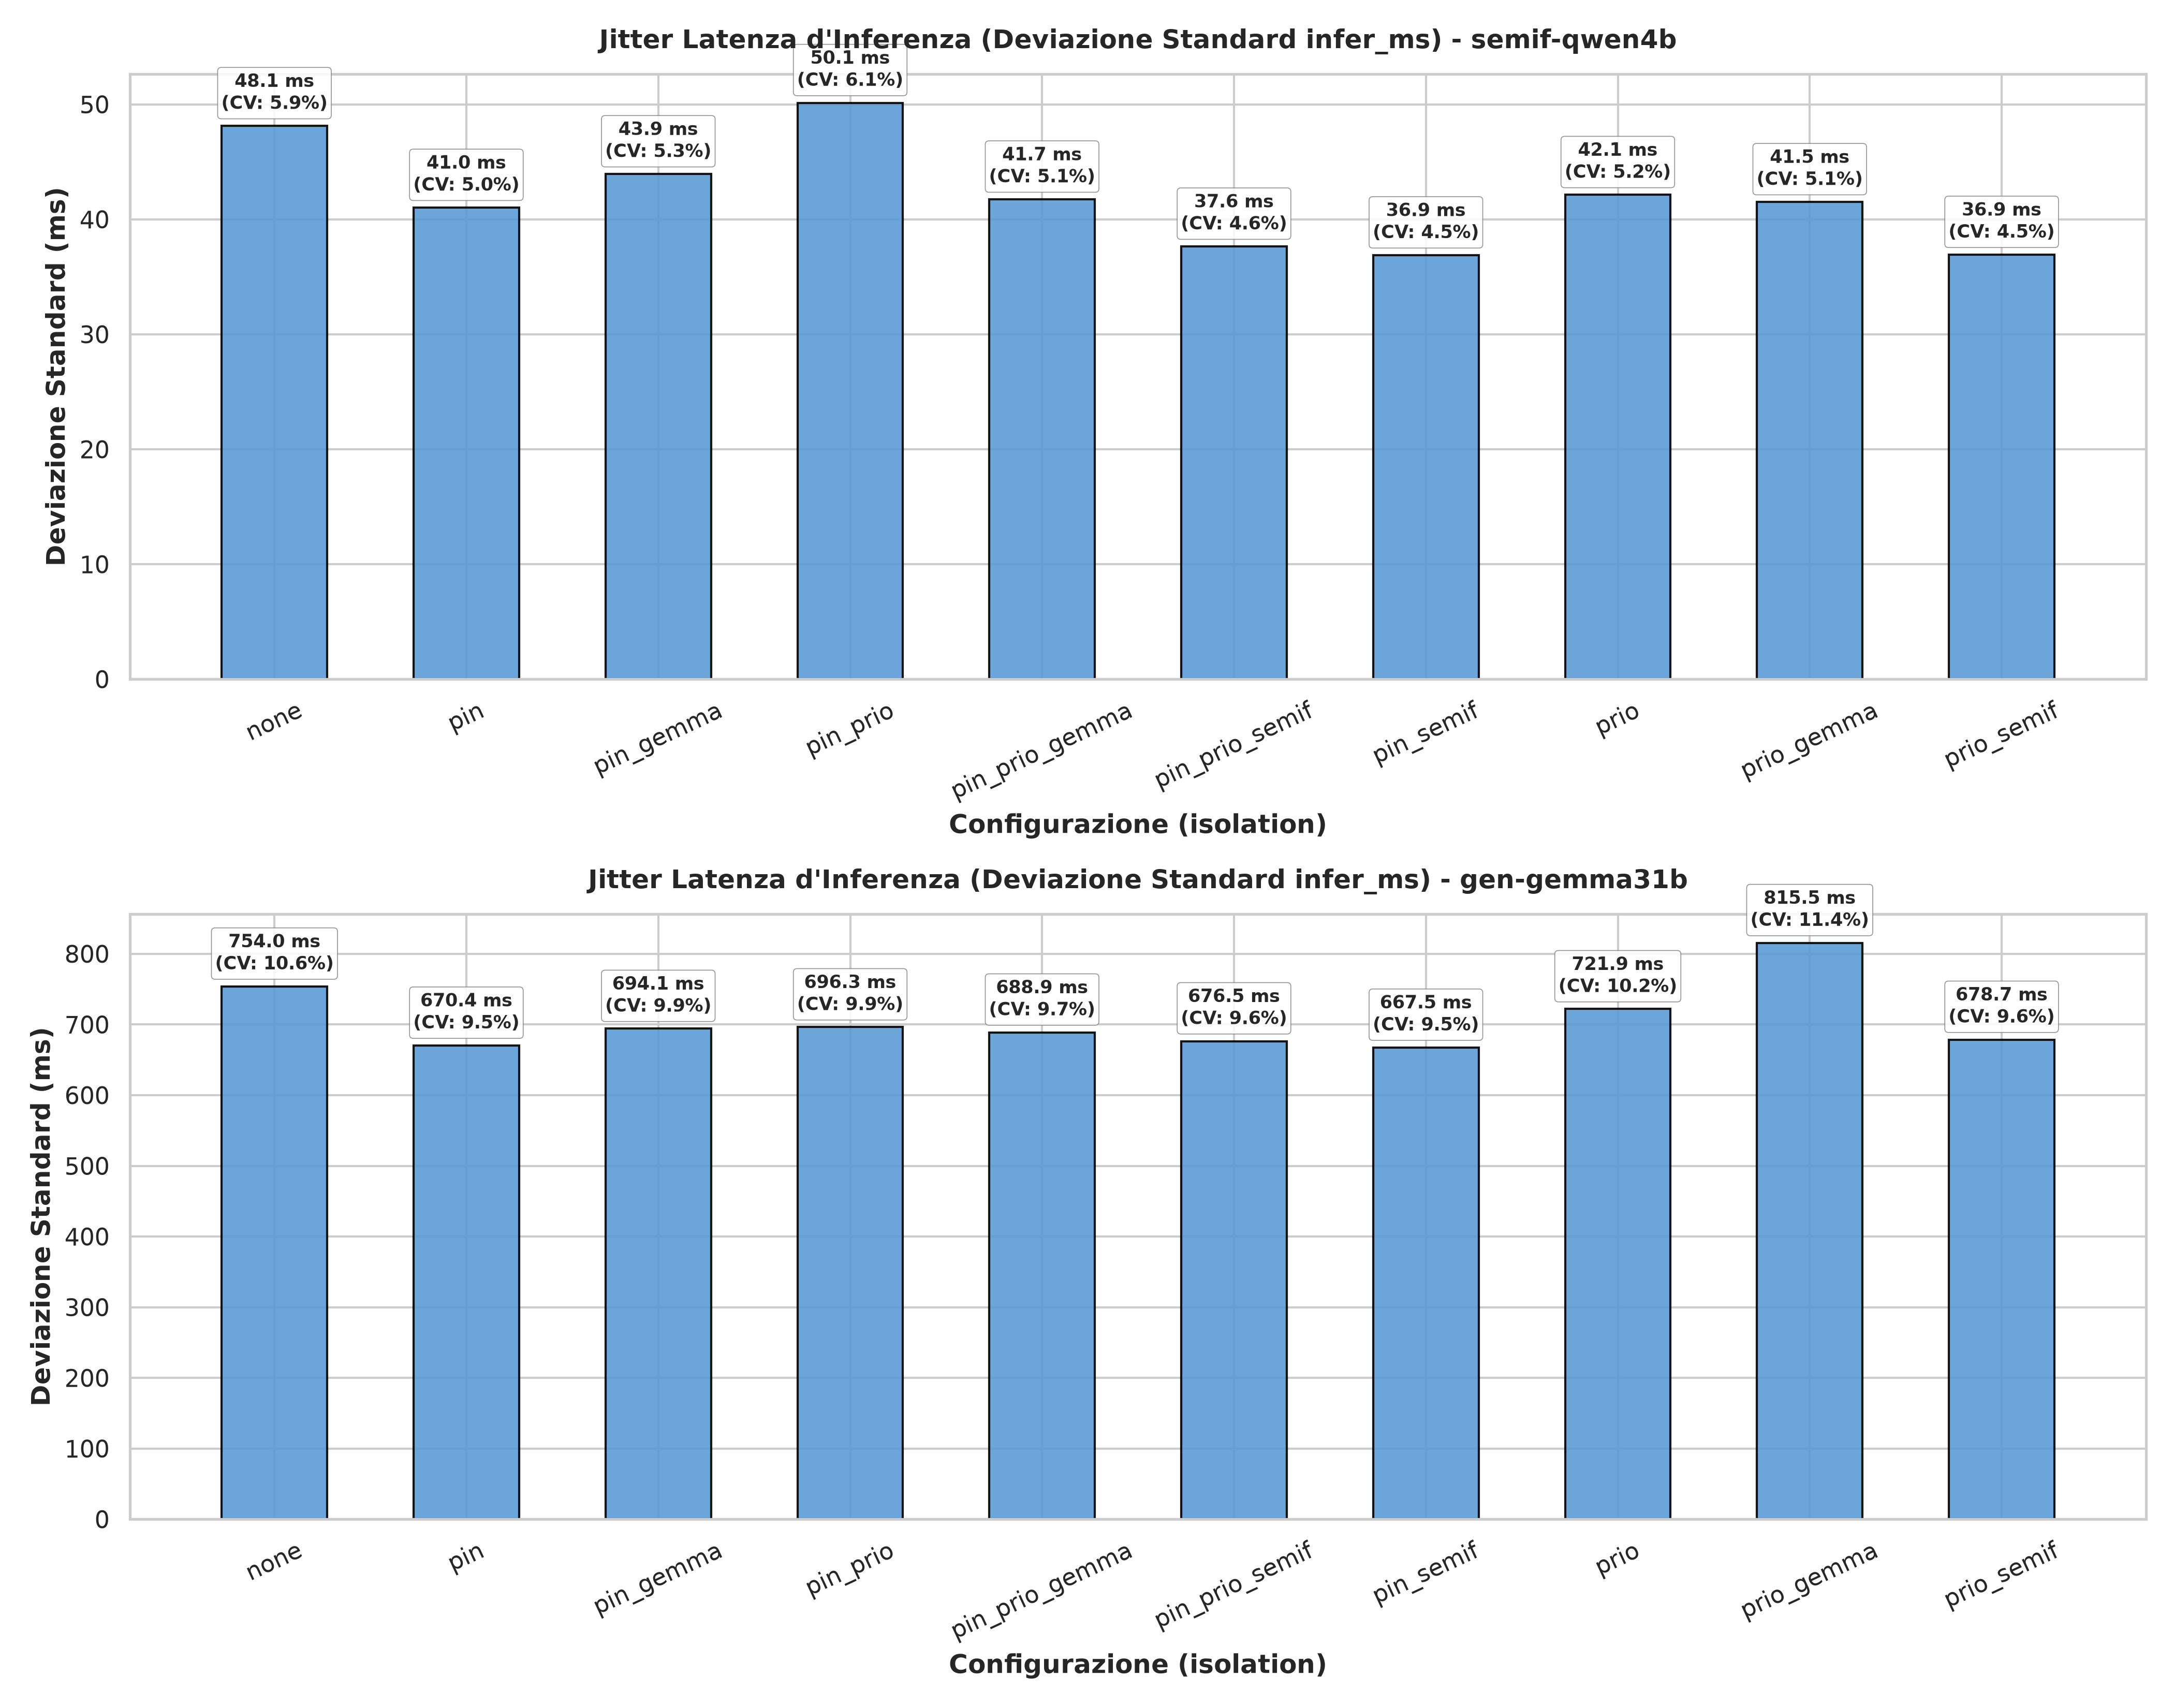
\includegraphics[width=0.97\columnwidth]{plots/markdown/b5_isolation_co_location/jitter_infer_ms.png}
\caption{B5: jitter e variabilità con isolamento in co-locazione.}\label{fig:b5jitter}
\end{figure}

\FloatBarrier
\subsection{Interpretazione dei risultati}
Il risultato è coerente con un limite delle strategie adottate: esse agiscono sull'esecuzione CPU e non assegnano quote o finestre esclusive di utilizzo della GPU. La contesa dell'acceleratore permane quindi anche quando i processi sono vincolati a core isolati.

\FloatBarrier
\section{Conclusioni}\label{sec:conclusions}

Il confronto sperimentale evidenzia un compromesso tra rapidità, stabilità e accuratezza. SemIf, con tempo di inferenza a riposo pari a circa 238 ms, risulta più rapido e presenta una variabilità assoluta inferiore rispetto a Gemma. Tale vantaggio è particolarmente rilevante per applicazioni embedded nelle quali l'output consiste nella selezione di un'azione tra alternative note. Le condizioni più sfavorevoli mostrano tuttavia un degrado significativo anche per SemIf, con latenze di coda fino a circa 1,4 s nei test di interferenza.
La selezione in un insieme finito semplifica il contratto di uscita, ma non esclude decisioni errate. Anche Gemma è invocato mediante uno schema JSON vincolato; la correttezza semantica e il rispetto delle scadenze devono dunque essere valutati separatamente dal formato della risposta. L'accuratezza inferiore osservata in alcuni casi per SemIf richiede ulteriori verifiche prima di un impiego nel controllo di sistemi reali.
Per Gemma, la generazione autoregressiva introduce una componente temporale aggiuntiva, sensibile alle risorse condivise. Il throughput complessivo a riposo è pari a circa 3,35 token/s. Il confronto non consente di separare gli effetti dell'architettura decisionale da quelli della dimensione dei modelli, della quantizzazione e dei backend.
Il pinning sui core isolati attenua le interferenze dei carichi CPU e risulta più efficace del solo incremento di priorità. In co-locazione, invece, l'isolamento della CPU non risolve la contesa della GPU. Il controllo dell'accesso all'acceleratore costituisce quindi una direzione di approfondimento per ottenere una maggiore prevedibilità.

La versione di SemIf impiegata in questo lavoro rappresenta soltanto una prima implementazione aperta dell'approccio System One e non esaurisce le possibilità del paradigma. L'ecosistema si sta sviluppando rapidamente e questi modelli sono oggi indicati anche con la denominazione \emph{decision models}, adottata da progetti quali Laya e Ollaya~\cite{laya,ollaya}. Laya propone un modello decisionale non autoregressivo basato su encoder, che restituisce decisioni tipizzate in un singolo passaggio. Il repository ufficiale riporta una latenza di 33 ms per una domanda su NVIDIA T4, quindi nell'ordine dei 30 ms~\cite{laya}. Il dato suggerisce un potenziale di riduzione dei tempi di inferenza rispetto alla prima implementazione qui valutata; hardware, carichi e protocolli differenti impediscono tuttavia un confronto diretto con i circa 238 ms misurati su Jetson AGX Orin e non consentono di dedurre un miglioramento dell'accuratezza. Parallelamente, Ollaya fornisce un motore per scaricare ed eseguire localmente decision models, incluso Laya, esponendoli tramite un servizio compatibile con l'interfaccia TypeSafe~\cite{ollaya}.

Ulteriori sviluppi comprendono la valutazione di questi modelli e motori sulla medesima piattaforma e con gli stessi carichi sperimentali, la specializzazione del modello decisionale mediante fine-tuning, il confronto con modelli generativi di dimensione comparabile e la misura dei messaggi scartati. Per valutare requisiti hard real-time occorrono inoltre scadenze esplicite, una caratterizzazione riproducibile del jitter e un'analisi del caso peggiore. La caratterizzazione della latenza di scheduling mediante \code{cyclictest} costituisce un ulteriore sviluppo della valutazione temporale. Le osservazioni presentate descrivono le configurazioni sperimentate e non forniscono garanzie temporali universali.

\FloatBarrier
\balance
\begin{thebibliography}{00}
\bibitem{typesafe} D. Almeida, ``Introducing System One Models \& Jev,'' TypeSafe AI, 15 settembre 2026. [Online]. Disponibile: \url{https://typesafe.ai/blog/introducing-system-one-models-and-jev}. Consultato il 15 ottobre 2026.
\bibitem{openjev} TheoLeeCJ e collaboratori, ``SemIf (formerly OpenJev),'' repository GitHub. [Online]. Disponibile: \url{https://github.com/TheoLeeCJ/SemIf-OpenJev}. Consultato il 15 ottobre 2026.
\bibitem{gemma-core} Google, ``Panoramica del modello Gemma 4,'' Google AI for Developers. [Online]. Disponibile: \url{https://ai.google.dev/gemma/docs/core?hl=it}. Consultato il 15 ottobre 2026.
\bibitem{gemma-card} Google DeepMind, ``Gemma 4 model card,'' Google AI for Developers. [Online]. Disponibile: \url{https://ai.google.dev/gemma/docs/core/model_card_4}. Consultato il 15 ottobre 2026.
\bibitem{openjev-method} TheoLeeCJ e collaboratori, ``Method,'' SemIf-OpenJev. [Online]. Disponibile: \url{https://github.com/TheoLeeCJ/SemIf-OpenJev/blob/master/docs/METHOD.md}. Consultato il 15 ottobre 2026.
\bibitem{laya} NandhaKishorM e collaboratori, ``Laya,'' repository GitHub. [Online]. Disponibile: \url{https://github.com/NandhaKishorM/laya}. Consultato il 18 ottobre 2026.
\bibitem{ollaya} M. Cobanov e collaboratori, ``Ollaya,'' repository GitHub. [Online]. Disponibile: \url{https://github.com/ollaya-dev/ollaya}. Consultato il 18 ottobre 2026.
\end{thebibliography}
\end{document}
